\documentclass[conference]{IEEEtran}

% --- Packages ---
\usepackage[T1]{fontenc}
\usepackage[utf8]{inputenc}
\usepackage{amsmath,amssymb}
\usepackage{graphicx}
\usepackage{booktabs}
\usepackage{url}
\usepackage{cite}
\usepackage{array}
\usepackage{multirow}
\usepackage{xcolor}
\usepackage{listings}
\usepackage{hyperref}

\lstset{
  basicstyle=\ttfamily\footnotesize,
  breaklines=true,
  frame=single,
  numbers=left,
  numberstyle=\tiny,
  xleftmargin=1.5em,
  framexleftmargin=1.5em
}

% IEEEtran citation style — must appear inside document body
% (placed before \bibliography below)

% -------------------------------------------------------
\begin{document}
\title{An empirical characterization of OpenMP loop scheduling policies: A case study in workload irregularity, spatial clustering and dispatch overhead}

\author{
    \IEEEauthorblockN{Gaurav Kapildeo Prasad (23BCE0449)}
    \IEEEauthorblockA{Case Study -- CS2 S01\\
    GitHub: \href{https://github.com/gaurav-k-prasad/Parallel-Computing-scheduling-study}{Repository Link}}
}



\maketitle

\begin{abstract}
The loop scheduling clause of OpenMP provides three main strategies (static, dynamic, and guided) along with a tunable parameter ``chunk size'' to control the granularity of the workload distribution. Although the approaches are popular in high-performance computing, we lack definitive/quantitative insights into when a strategy should be preferred over the others, and such guidelines are often anecdotal. This paper reports a controlled empirical study on all three approaches across 6 workload profiles, 5 thread counts, 3 chunk sizes, and 2,492 measured exec records on AMD Ryzen 7 6800H (8 physical cores, 16 simultaneous multithreading, SMT threads). Our major findings are as follows. (1) We show that the geometry of how computation is spatially distributed over iteration index space can make a significant difference (\(\times 2\) or more) to the performance of static scheduling (under fixed CV and strict total workload) which cannot be predicted by just CV alone. (2) We characterize the dispatch overhead using low-work probe approach and found that dynamic (with unit chunks, \(C=1\)) suffers 8.3\% regression on perfect regular loops at 16 threads (due to atomic queueing contention), while dynamic (\(C=8\)) outperforms the default (static) up to 67.4\% on spatially clustered irregular loops. (3) We validate the synthetic results on a real-world Mandelbrot fractal (\(1200\times900\), \(CV\approx1.65\)), where we see \(9.55\times\) speedup (vs 5.13\(\times\) for default, static) with dynamic (\(C=8\)). All source code, raw data, and analysis scripts are available at the companion repository.
\end{abstract}

\begin{IEEEkeywords}
OpenMP, loop scheduling, dynamic scheduling, guided scheduling, load balancing, workload irregularity, parallel efficiency, dispatch overhead, Mandelbrot, empirical study
\end{IEEEkeywords}

\section{Introduction}

The selection of a parallel loop scheduling policy is one of the most important decisions to be taken in order to parallelise a computationally intensive loop using OpenMP. The selected scheduling policy determines the allocation of the \(N\) iterations of the loop to \(P\) threads and thus determines the level of achieved load balancing and the overheads of coordination. In the case where all iterations have the same cost, the practically optimal approach is the static assignment using a block partitioning with \(\lceil N/P\rceil\) size. In this case, all threads are allocated the same amount of work with a zero dispatch overhead at runtime. On the other hand, in the case of different cost for the iterations, the static assignment may result in some threads being idle at the synchronisation barrier while others are still running, and this may negatively affect the achieved speedup and efficiency.

Dynamic and guided scheduling are tackling these problems by postponing iteration assignment to runtime. Threads grab chunks of work from the shared queue on-the-fly, naturally moving load from fast to slow threads. This comes at the price of synchronisation overhead, where each chunk of work grabbing requires an atomic counter or spinlock operation on the shared queue. This can dominate the actual computation if per-iteration work is small or if we have lots of threads (\(C=1\)).

As such, tradeoffs related to the ones discussed above have been studied since the 80s \cite{kruskal1985allocating,polychronopoulos1987guided,tang1986processor}. However, it is not well-systematised (a) to the point where we see how precisely workload irregularity and space-distribution of iteration costs (rather than variance) are interacting, (b) where we see how varying chunk size affects dispatch overhead at realistic thread counts for a modern AMD Zen 3+ processor when running under SMT, or (c) if we can take what we learned from synthetic-type benchmarks and apply it to a real scientific application kernel. We aim to fill all these gaps by means of a factorial study experiment that is a fully self-contained C++17/OpenMP code base with full Python-based analysis infrastructure.

The structure of the rest of the paper is as follows. In Section Background and Related Work we discuss related work in the field of loop scheduling. In Section Formulation we state the experimental hypotheses and evaluation criteria. In Section Architecture we present system architecture. In Section Implementation we describe workload generator, scheduling dispatcher and Mandelbrot benchmark implementation. In Section Evaluation we show the experimental setup and the results. We discuss the findings and their implications in Section Discussion. In Section Limitations we point out the limitations and future work. Section Conclusion concludes.

\section{Background and Related Work}

\subsection{Basic Concepts of Loop Scheduling}

The concept of static scheduling pre-dates the standard. In the early 1980s, Kruskal and Weiss \cite{kruskal1985allocating} studied a problem of distributing independent tasks across processors. They laid the theoretical foundations for both block and cyclic assignment schemes. Static block scheduling is about minimising the coordination cost with the assumption of uniform load. Cyclic (or round-robin) allocation is about the amortisation of irregularity but with a loss in terms of spatial locality. In OpenMP, these concepts are formalised as \texttt{schedule(static)} with or without an explicit chunk size \cite{openmp2021spec52}.

The guided self-scheduling method proposed by Polychronopoulos and Kuck \cite{polychronopoulos1987guided} for shared memory multiprocessor. The main idea was to use large chunks early on (to reduce queue transactions if a lot of iteration space remains) and smaller ones towards the end (to make sure that stragglers do not introduce a large delay to the barrier). A related set of policies for partitioning the iteration space called factoring was introduced by Hummel et al. \cite{hummel1992factoring}. The idea was to decompose the iteration space into phases and take \(1/(2P)\) of the remaining work for each phase. In both cases, they take advantage of the fact that the expected makespan is minimized when the expected load on each thread is equal to the ideal balanced load. Work stealing type of schedulers, popularized by the Cilk scheduler \cite{blumofe1999scheduling,agrawal2010cilk} have the complementary strategy of having idle threads steal pending work from busy ones. This has very strong theoretical bounds but comes with the drawback of having more complex runtime support as compared to the centralized queue used in OpenMP dynamic scheduling.

Analytical models of loop decompositions for variable iteration execution time was studied by Liou and Pitsianis \cite{liou1997hyperbolic}. Empirical classifications of loop parallelism for a variety of scientific applications domains was studied by Tzenakis et al. \cite{tzenakis2012bddt}.

\section{OpenMP Runtime Implementations and Measuring Overheads}

Early work on measuring the cost of synchronisation and scheduling overheads with OpenMP runtimes was done by Bull~\cite{bull1999measuring}, who measured the costs of dynamic scheduling in terms of tens of microseconds per synchronisation event for hardware of the time. For a comprehensive reference to portable programming in OpenMP, with semantics of \texttt{schedule(runtime)} and interplay between \texttt{OMP\_SCHEDULE} environment variables and \texttt{omp\_set\_schedule()}, see Chapman et al.~\cite{chapman2007using}.

More recent work by Duran et al.~\cite{duran2008openmp} performed a comparison of different OpenMP scheduling approaches across multiple applications and runtime implementations, which also showed that the optimal policy selection is application/architecture dependent. EPCC OpenMP microbenchmarks~\cite{markbull2001epcc} provided a repeatable methodology to measure loop scheduling overheads, which we extend here. Finally, Eachempati and Chapman~\cite{eachempati2010evaluating} studied OpenMP tasking and work-sharing approaches for irregular applications, where it was shown that task decomposition can be superior to loop-level dynamic scheduling for highly irregular workloads in tree-structured data (a complementary finding to ours).

\subsection{Positioning of This Work}

Most empirical work in the past has considered one or two cases of workload profile or does not explicitly separate the spatial arrangement of workload from total variation. Here, we have developed a controlled synthetic benchmark which keeps an identical multiset of per-iteration costs (and hence CV) constant between two cases of experiment while varying only the spatial arrangement of such costs for clear separation of the effect of load correlation structure versus magnitude of irregularity.

\section{Problem Formulation and Research Questions}

\subsection{Formal Statement of Problem}

A parallel loop of \(N\) iterations with a computational cost \(W_i > 0\) for iteration \(i\), executed by \(P\) threads. The scheduling policy organizes a series of non-overlapping chunked work \(\{C_1, C_2, \ldots\}\) to be allocated for the ready threads. The target dependent variable to be measured is parallel wall-clock execution time \(T(N, W, \text{policy}, C, P)\) as measured by \texttt{omp\_get\_wtime()}.

Derive three kinds of aggregate measures:

\begin{equation}
S_p = \frac{\widetilde{T}_{\text{serial}}}
{\widetilde{T}_{\text{parallel}}}
\end{equation}

\begin{equation}
E_p = \frac{S_p}{P}
\end{equation}

\begin{equation}
\Delta T_{\text{rel}} =
\frac{\widetilde{T}_{\text{static}} -
\widetilde{T}_{\text{policy}}}
{\widetilde{T}_{\text{static}}}
\times 100\%
\end{equation}

where the median for \(k=7\) is denoted by \(\widetilde{T}\), \(\widetilde{T}_{\text{serial}}\) is the median execution time for the serial version without OpenMP directives, and \(\widetilde{T}_{\text{static}}\) is the median for the default static policy with the same number of threads.

\subsection{Research Questions and Hypotheses}

There are five directional hypotheses:

\begin{itemize}
    \item \textbf{H1 [Static on Regular]:} Default static scheduling is competitive with regular workloads (\(\mathrm{CV}=0\)) by avoiding runtime dispatch coordination.

    \item \textbf{H2 [Dynamic on Irregular]:} Dynamic is superior to static when its gain in load balance outweighs the cost for dispatch contention.

    \item \textbf{H3 [Guided Trade-off]:} Guided offers a trade-off between early big chunks and late small chunks, but it is a function of workload spatial structure.

    \item \textbf{H4 [Spatial Arrangement]:} In case of spatial clustering of costly iterations, static is affected regardless of the workload's CV and thus CV alone is not a sufficient predictor of schedulability.

    \item \textbf{H5 [Chunk Contention]:} Unit chunk size (\(C=1\)) offers maximum load balance, but high atomic queue contention. \(C=8\) is a more reasonable operational point (medium size).
\end{itemize}

\subsection{Evaluation Criteria}

The results of a configuration are considered to outperform the static default if the 95\% bootstrap confidence interval for \(\Delta T_{\text{rel}}\) is positive. Speedup values are interpreted with respect to the ideal linear reference \(S_p=P\).

\section{System Architecture}

We implemented our study as a three-level system with (1) a compiled C++17 benchmark executable, (2) orchestration and analysis with Python, and (3) verification artefacts. See Fig.~\ref{fig:arch} for the architecture of the components.

\begin{enumerate}
    \item \textbf{Layer 1: Experiment Orchestrator} (\texttt{scripts/run\_experiments.py}, Python 3.12)
    \begin{itemize}
        \item Full \(6 \times 10 \times 5\) factorial matrix (300 parallel configurations).
        \item Pseudorandomized ordering for runs within one repetition (seed \(42 \oplus \text{rep index}\)).
        \item Invokes \texttt{build/benchmark} as a subprocess.
    \end{itemize}
\end{enumerate}

\begin{center}
\(\downarrow\) subprocess (CLI) \(\downarrow\)
\end{center}

\begin{enumerate}
    \setcounter{enumi}{1}
    \item \textbf{Layer 2: Benchmark Executable} (\texttt{build/benchmark}, C++17/OpenMP 4.5)
    \begin{itemize}
        \item \textbf{WorkloadGenerator} (\texttt{benchmark\_support.hpp}): \texttt{REGULAR}, \texttt{RANDOM\_LOW}, \texttt{RANDOM\_MED}, \texttt{RANDOM\_HIGH}, \texttt{CLUSTERED\_HIGH}, \texttt{MANDELBROT}.
        \item \textbf{SchedulingDispatcher}: \texttt{static\_default}, static/dynamic/guided \(\times C \in \{1,8,64\}\) (10 policies total).
        \item \textbf{ChecksumVerifier}: 64-bit FNV-1a hash for the output array, to guarantee correctness.
        \item \textbf{Timer}: \texttt{omp\_get\_wtime()}, roughly 10 ns resolution wall-clock.
    \end{itemize}
\end{enumerate}

\begin{center}
\(\downarrow\) \texttt{raw\_runs.csv} (2492 entries) \(\downarrow\)
\end{center}

\begin{enumerate}
    \setcounter{enumi}{2}
    \item \textbf{Layer 3: Analysis Pipeline} (\texttt{scripts/analyse\_results.py}, Python 3.12 + NumPy + pandas)
    \begin{itemize}
        \item Computes median, mean, standard deviation, and bootstrap confidence intervals (\(B=2000\), non-parametric, 95\%).
        \item Computes \(S_p\), \(E_p\), and \(\Delta T_{\text{rel}}\) (speedup \(S_p\)).
        \item Produces 10 publication figures in PNG (300 DPI) and vector PDF formats.
    \end{itemize}
\end{enumerate}

\begin{figure}[htbp]
    \centering
    \caption{Three-layer structure of the benchmark framework. Each layer has a single responsibility: the orchestrator drives the factorial sweep, the benchmark executable is responsible for timing and correctness, and the analysis pipeline is responsible for deriving all the statistics and figures from the raw CSV output.}
    \label{fig:arch}
\end{figure}

\subsection{Module Responsibilities}

\textbf{Workload Generator} (\texttt{benchmark\_support.hpp}, \texttt{generate\_synthetic\_workload}): Generates an integer cost vector \(W[0 \ldots N-1]\) before the timed region to ensure no allocation interference during the measurement. The generator takes as arguments a \texttt{WorkloadProfile} enum, \(N\) iterations, \(W_{\text{base}}\) for the base work, and a 64-bit seed to generate a repeatable cost vector, with the sum of the vector being exactly \(N \times W_{\text{base}}\).

\textbf{Scheduling Dispatcher} (\texttt{run\_synthetic\_parallel}, \texttt{run\_mandelbrot\_parallel}): Sets the OpenMP scheduling policy at runtime using \texttt{omp\_set\_schedule()}. Runs the work-sharing loop under \texttt{schedule(runtime)}. For default static scheduling, uses a compile-time \texttt{schedule(static)} directive to prevent any call to the runtime scheduler.

\textbf{Dispatch Probe} (\texttt{run\_probe\_parallel}): A minimal-work loop that runs the same iteration space with the same scheduling parameters but negligible per-iteration arithmetic cost. Isolates the coordination overhead from useful computation.

\textbf{Checksum Verifier} (\texttt{compute\_checksum}): Runs a 64-bit FNV-1a checksum on the output array at the end of each timed region. If all serial and parallel runs of the workload have the same checksum, then the result is deterministically correct.

\textbf{Experiment Orchestrator} (\texttt{run\_experiments.py}): Creates the full factorial cross-product of all 300 parallel configuration options, pseudorandomly shuffles the order within each repetition to avoid systematic drift, runs warmup and measured runs, and writes CSV rows into \texttt{results/raw/raw\_runs.csv}.
\textbf{Analysis Pipeline} (\texttt{analyze\_results.py}): Loads raw CSV data into a DataFrame (\texttt{pandas}), calculates median, mean, standard deviation, and 2000-bootstrap 95\% confidence intervals, derives speedup and efficiency, and generates 10 figures for publication (300 DPI PNG and vector PDF).

\section{Implementation and Methodology}

\subsection{Workload Generation with Controlled Irregularity}

The same total computational budget is maintained for all synthetic profiles:

\begin{equation}
B = \sum_{i=0}^{N-1} W_i
= N \times W_{\text{base}}
= 50{,}000{,}000
\label{eq:budget}
\end{equation}

with \(N = 100{,}000\) and \(W_{\text{base}} = 500\).

This invariant enables direct performance comparison between profiles, since every thread should collectively execute the same total amount of arithmetic work.

\subsubsection{Regular Workload}

All iterations have a cost of \(W_{\text{base}}\), resulting in exactly \(\mathrm{CV} = 0\). This case is deterministic, uses a single code path, and requires no sampling.

\subsubsection{Randomized Irregularity}

Continuous samples \(X_i \sim \Gamma(k,1)\) are generated using \texttt{std::mt19937\_64}, seeded at \(S = 42\).

The Gamma shape parameter \(k = 1/\mathrm{CV}^2\) relates the target irregularity levels to the distribution. The values are \(k = 16\) for \(\mathrm{CV} = 0.25\), \(k = 4\) for \(\mathrm{CV} = 0.50\), and \(k = 1\) (exponential distribution) for \(\mathrm{CV} = 1.00\).

The raw variates are scaled to the budget \(B\):

\begin{equation}
Y_i = \frac{X_i}{\sum_j X_j} \times B
\label{eq:scale}
\end{equation}

Integer costs \(W_i = \max(1,\lfloor Y_i \rfloor)\) are then adjusted using deterministic distribution of the integer excess or deficiency by means of fractional-remainder sorting, ensuring that

\[
\sum_{i=0}^{N-1} W_i = B.
\]

\subsubsection{Clustered Irregularity}

For the \(\mathrm{CV} = 1.00\) randomized profile, the resulting integer vector is sorted in ascending order. The top 50\% of the sorted list's costliest iterations are placed contiguously in the central region \([N/4, 3N/4)\), while the bottom 50\% are placed in the outer flanks.

This is a pure permutation of the randomized array. The multiset, histogram, mean, variance, and CV are strictly identical to the randomized case, as verified by the correctness test suite. Thus, any performance difference between this pair of profiles is solely due to spatial work correlation.

\subsection{Synthetic Kernel}

A fixed number of 64-bit integer mixing steps are applied to a loop-carried state, initialized per iteration using the loop index, in the inner loop body:

\begin{lstlisting}[language=C++,
    caption={Synthetic hash kernel executed W[i] times per iteration.},
    basicstyle=\ttfamily\small,
    numbers=left,
    frame=single]
uint64_t state =
    (uint64_t)i ^ 0x9e3779b97f4a7c15ULL;

for (uint32_t step = 0; step < W[i]; ++step)
{
    state ^= (state >> 30);
    state *= 0xbf58476d1ce4e5b9ULL;
    state ^= (state >> 27);
    state *= 0x94d049bb133111ebULL;
    state ^= (state >> 31);
    state += step;
}
out[i] = state;
\end{lstlisting}

The good things about this kernel is that:

\begin{enumerate}
    \item The state dependent loop carried dependency prevents the compiler from applying any closed form simplifications, making sure all of the $W_i$ mixing actually happens.

    \item It has one write per element per iteration (no false sharing without padding).

    \item It is completely ALU bound and doesn't have any mem allocation. Hence shielding it from variability in the memory system that could affect the scheduling.
\end{enumerate}

\subsection{Implementation of Scheduling}

OpenMP has three runtime schedulers via the \texttt{schedule} clause \cite{openmp2021spec52}. Four element \texttt{SchedPolicy} enum are exposed at the implementation level:

\begin{enumerate}
    \item \texttt{STATIC\_DEFAULT}: \texttt{\#pragma omp parallel for} with static scheduling in compile time (without chunksize). The openMP runtime splits $N$ iterations evenly to $P$ contiguous blocks of size $\lceil N/P \rceil$. There is no runtime queue involved.

    \item \texttt{STATIC\_CHUNK}: \texttt{omp\_set\_schedule} at runtime (configurible). The assignment of iterations to threads using cyclic round robin ($C$ sized chunk), a coordination step is needed. But with very low overhead per chunk.

    \item \texttt{DYNAMIC\_CHUNK}: \texttt{omp\_sched\_dynamic} (with size $C$). The next available $C$ sized chunk of iterations is atomically obtained by each thread from the shared counter (work stealing variant).

    \item \texttt{GUIDED\_CHUNK}: \texttt{omp\_sched\_guided} (with minimum chunk size $C$). The assigned chunk size gets reduced by the following (roughly)

    \[
    \max(C,\lfloor \text{remaining}/P\rfloor)
    \]

    on each dispatch.
\end{enumerate}

If we use chunked policies then we use \texttt{schedule(runtime)} (after \texttt{omp\_set\_schedule}). Together, these offer the possibility to reuse code (not duplicate) for a single loop body that can be tuned dynamically.

Each timed region starts with \texttt{omp\_set\_dynamic(0)} to disable dynamic thread control. We use environment variables (\texttt{OMP\_DYNAMIC=FALSE}, \texttt{OMP\_PLACES=cores}, \texttt{OMP\_PROC\_BIND=close}) to guarantee thread affinity and bind threads to physical cores in a "close" binding policy.

\subsection{Mandelbrot Domain Benchmark}

The Mandelbrot computation \cite{mandelbrot1980fractal} calculates the escape time function for all points $c = x_0 + i y_0$ ($x \in [-2.0, 0.5]$, $y \in [-1.25, 1.25]$) on a $1200 \times 900$ grid, up to a maximum number of iterations = 400.

This is flattened into a single 1D loop with $N=1080000$ number of iterations. The number of escape iterations per pixel can vary from 1 (points that escape immediately) to 400 (points on/inside the boundary of the Mandelbrot). The value for CV is $\sim 1.65$. It's the most irregular of all profiles in our study.

The benchmark, unlike the synthetic kernel, offers naturally heterogeneous, spatially structured fractal geometry. It is a nice external validity check.

\subsection{Dispatch Overhead Probe}

To measure the actual overhead of OpenMP scheduling directly, either performance counters from the hardware or tracing (not available through portable OpenMP calls). So what we do is use a light-weight probe loop with the same iteration space, chunk setup and number of threads as the corresponding workload measuring part but with minimal arithmetic work per iteration like the following:

\[
\texttt{out[i]} = (\texttt{i} * \texttt{3141592653589793238ULL})
\]

\[
\texttt{XOR 0x5a5a5a5a5a5a5a5aULL}
\]

which has a single integer multiply-xor to do. So the useful work per iteration is $O(1)$ ALU cycles. This way the probe runtime mainly accounts for the entry/exit of the parallel region, synchronization between threads, atomic chunk queue operations, barrier latencies etc., so it is a low-bound surrogate for the pure dispatch overhead.

\section{STATISTICAL ANALYSIS}

We use the robust estimator of repeated measurements $T_1, \ldots, T_7$, the sample median $\tilde{T}$,
mean, and standard deviation. Sample medians are used to calculate the speedup ($S_p$),
relative improvement ($D_{\mathrm{rel}\ T}$). Equations (speedup),(relative improvement).

$B = 2000$ bootstrap samples (sample with replacement) for non-parametric confidence intervals. We use a joint sampling of series and parallel reps vector to preserve the correlation structure of the ratio for speedup ratios.

\[
S_{p,b}^{*} = \frac{T_{s,b}^{*}}{T_{p,b}^{*}}, \quad b = 1, \ldots, B
\]

95\% - by 2.5 and 97.5 percentile of bootstrap speed-up value

\section{Experimental Setup \& Evaluation}

\subsection{Hardware/Software}

Hardware/Software for experiment

\begin{table}[htbp]
\centering
\begin{tabular}{ll}
\hline
\textbf{component} & \textbf{Specification} \\
\hline
Processor & AMD Ryzen 7 6800H (Zen 3+ Rembrandt 6nm) \\
Phys. cores & 8 (Smt 2 thread/core) \\
Logical processors & 16 \\
Base/boost clock & 3.2GHz / 4.7GHz \\
L1d/l1i cache & 8*32KiB/8*32KiB \\
L2 cache & 8*512KiB \\
L3 cache & 16Mib (1*shared) \\
NUMA node & 1 \\
System memory & 7.4GiB (WSL2 all. mem) \\
OS/kernel & ubuntu 24.04 lts. Linux 6.6.87.1-wsl2 \\
Compiler & g++ 13.3.0 (opt -O3) cpp17 \\
OpenMP runtime & GNU libgomp (openmp 4.5/spec 201511) \\
Thread affinity & OMP\_PLACES=cores, OMP\_PROC\_BIND=close \\
Python stack & python 3.12.7, NumPy 1.26.4, pandas 2.2.2 \\
\hline
\end{tabular}
\end{table}

Full experiment environment (that is captured in results/raw/environment.json by run of benchmarks) is captured by table (tab:env)

We are using single-socket desktop APU with a virtualization component by (Winodws Subsystem for Linux) WSL2 as host (which effects timing jitters that mitigated by run order randomisation and non-paramertic stats).

\subsection{Experiment Matrix}

We have full factorial cross-product of

\begin{itemize}
    \item 6 work load profiles: reg(CV=0), random\_low(CV$\sim$0.25), random\_med(CV$\sim$0.50), random\_high(CV$\sim$1.00), clusterd\_high(CV$\sim$1.00 but spatially permuted), mandelbrot(CV$\sim$1.65)
    \item 10 scheduling configs: static\_default, static, dynamic, guided, all for $C \in \{1, 8, 64\}$
    \item 5 \#threads: $P \in \{1, 2, 4, 8, 16\}$
    \item 5 measurements per cell (plus 1 for warm-up)
\end{itemize}

add'l 392 rows for serial baselines (6wks x 7reps) + dispatch probe measurements (10 scheds x 5ths x 7reps) completeness of the \#records total measurement 2492 verified by script \texttt{/s/validate\_results.py} 100\% checksum (deterministic) consistency across all configs for major workload characteristics for each workload. summarised in table (tab:workloads) 100\% checksums (deterministic) across all configs verified by script \texttt{/s/validate\_results.py}

\begin{table*}[t]
\centering
\caption{Workload profile summary n = 100,000 w\_base = 500 seed = 42}
\label{tab:workloads}
\begin{tabular}{l l c c r r r r}
\hline
\textbf{Profile} & \textbf{Arrangement} & \textbf{Target CV} & \textbf{Actual CV} & \textbf{n (iterations)} & \textbf{Total work} & \textbf{Serial t (msec)} & \textbf{Sigma serial (msec)} \\
\hline
regular & uniform & 0.00 & 0.0000 & 100,000 & 50,000,000 & 272.3 & 4.76 \\
random low & randomised & 0.25 & 0.2501 & 100,000 & 50,000,000 & 275.8 & 5.44 \\
random med & randomised & 0.50 & 0.5001 & 100,000 & 50,000,000 & 277.0 & 4.35 \\
random high & randomised & 1.00 & 1.0035 & 100,000 & 50,000,000 & 276.7 & 6.03 \\
clustered high & clustered & 1.00 & 1.0035 & 100,000 & 50,000,000 & 273.1 & 1.59 \\
mandelbrot & fractal geom. & & 1.6504 & 1,080,000 & 110,709,598 & 479 & \\
\hline
\end{tabular}
\end{table*}

Individual cells are invoked from separate build/benchmark subprocesses. All 300 parallel configurations are shuffeled pseudo-randomly for every repetition $r \in \{0, \ldots, 6\}$ (seed: $S = 42$ with per-repetition index perturbation) to avoid correlation of thermal bias and frequency boost decay effects with policy type. A single untimed warm-up run is performed before measuring to initialise OpenMP thread pool and processor frequency state. Measurement of execution time is performed by \texttt{omp\_get\_wtime()} with $\sim$10 ns resolution on this platform (far below 20-280ms measurement range).

\subsection{Key Findings on Timing}

The key findings are shown in the table (tab:main-results) at max. concurrency of the evaluation platform (16 threads). Median runtimes are given with 95\% bootstrap confidence intervals.

\begin{table}[htbp]
\centering
\caption{Median Runtime (ms) at 16 threads (95\% Bootstrap CI)}
\label{tab:main-results}
\resizebox{\columnwidth}{!}{%
\begin{tabular}{llrrl}
\hline
\textbf{Workload \& Policy} & & $\tilde{T}$ (ms) & $S_p$ & $\Delta T_{\mathrm{rel}}$ \\
\hline
Regular (CV=0.00) & static\_default & 33.75 & 8.07$\times$ & Baseline \\
 & dynamic\_c1 & 36.55 & 7.45$\times$ & -8.3\% \\
 & dynamic\_c8 & 27.95 & 9.74$\times$ & +17.2\% \\
 & guided\_c8 & 28.74 & 9.48$\times$ & +14.8\% \\
\hline
Random High (CV=1.00) & static\_default & 34.05 & 8.13$\times$ & Baseline \\
 & dynamic\_c1 & 23.64 & 11.71$\times$ & +30.6\% \\
 & dynamic\_c64 & 23.42 & 11.82$\times$ & +31.2\% \\
 & guided\_c1 & 22.86 & 12.10x & +32.8\% \\
\hline
Clustered High (CV = 1.00) & static\_default & 69.43 & 3.93x & Baseline \\
 & static\_c1 & 26.91 & 10.15x & +61.2\% \\
 & dynamic\_c1 & 26.52 & 10.30x & +61.8\% \\
 & dynamic\_c8 & 22.60 & 12.08x & +67.4\% \\
\hline
Mandelbrot (CV $\sim$ 1.65) & static\_default & 93.41 & 5.13x & Baseline \\
 & dynamic\_c1 & 72.90 & 6.57x & +22.0\% \\
 & dynamic\_c8 & 50.13 & 9.55x & +46.3\% \\
 & guided\_c1 & 82.58 & 5.80x & +11.6\% \\
\hline
\end{tabular}%
}
\end{table}

\begin{figure}[htbp]
\centering
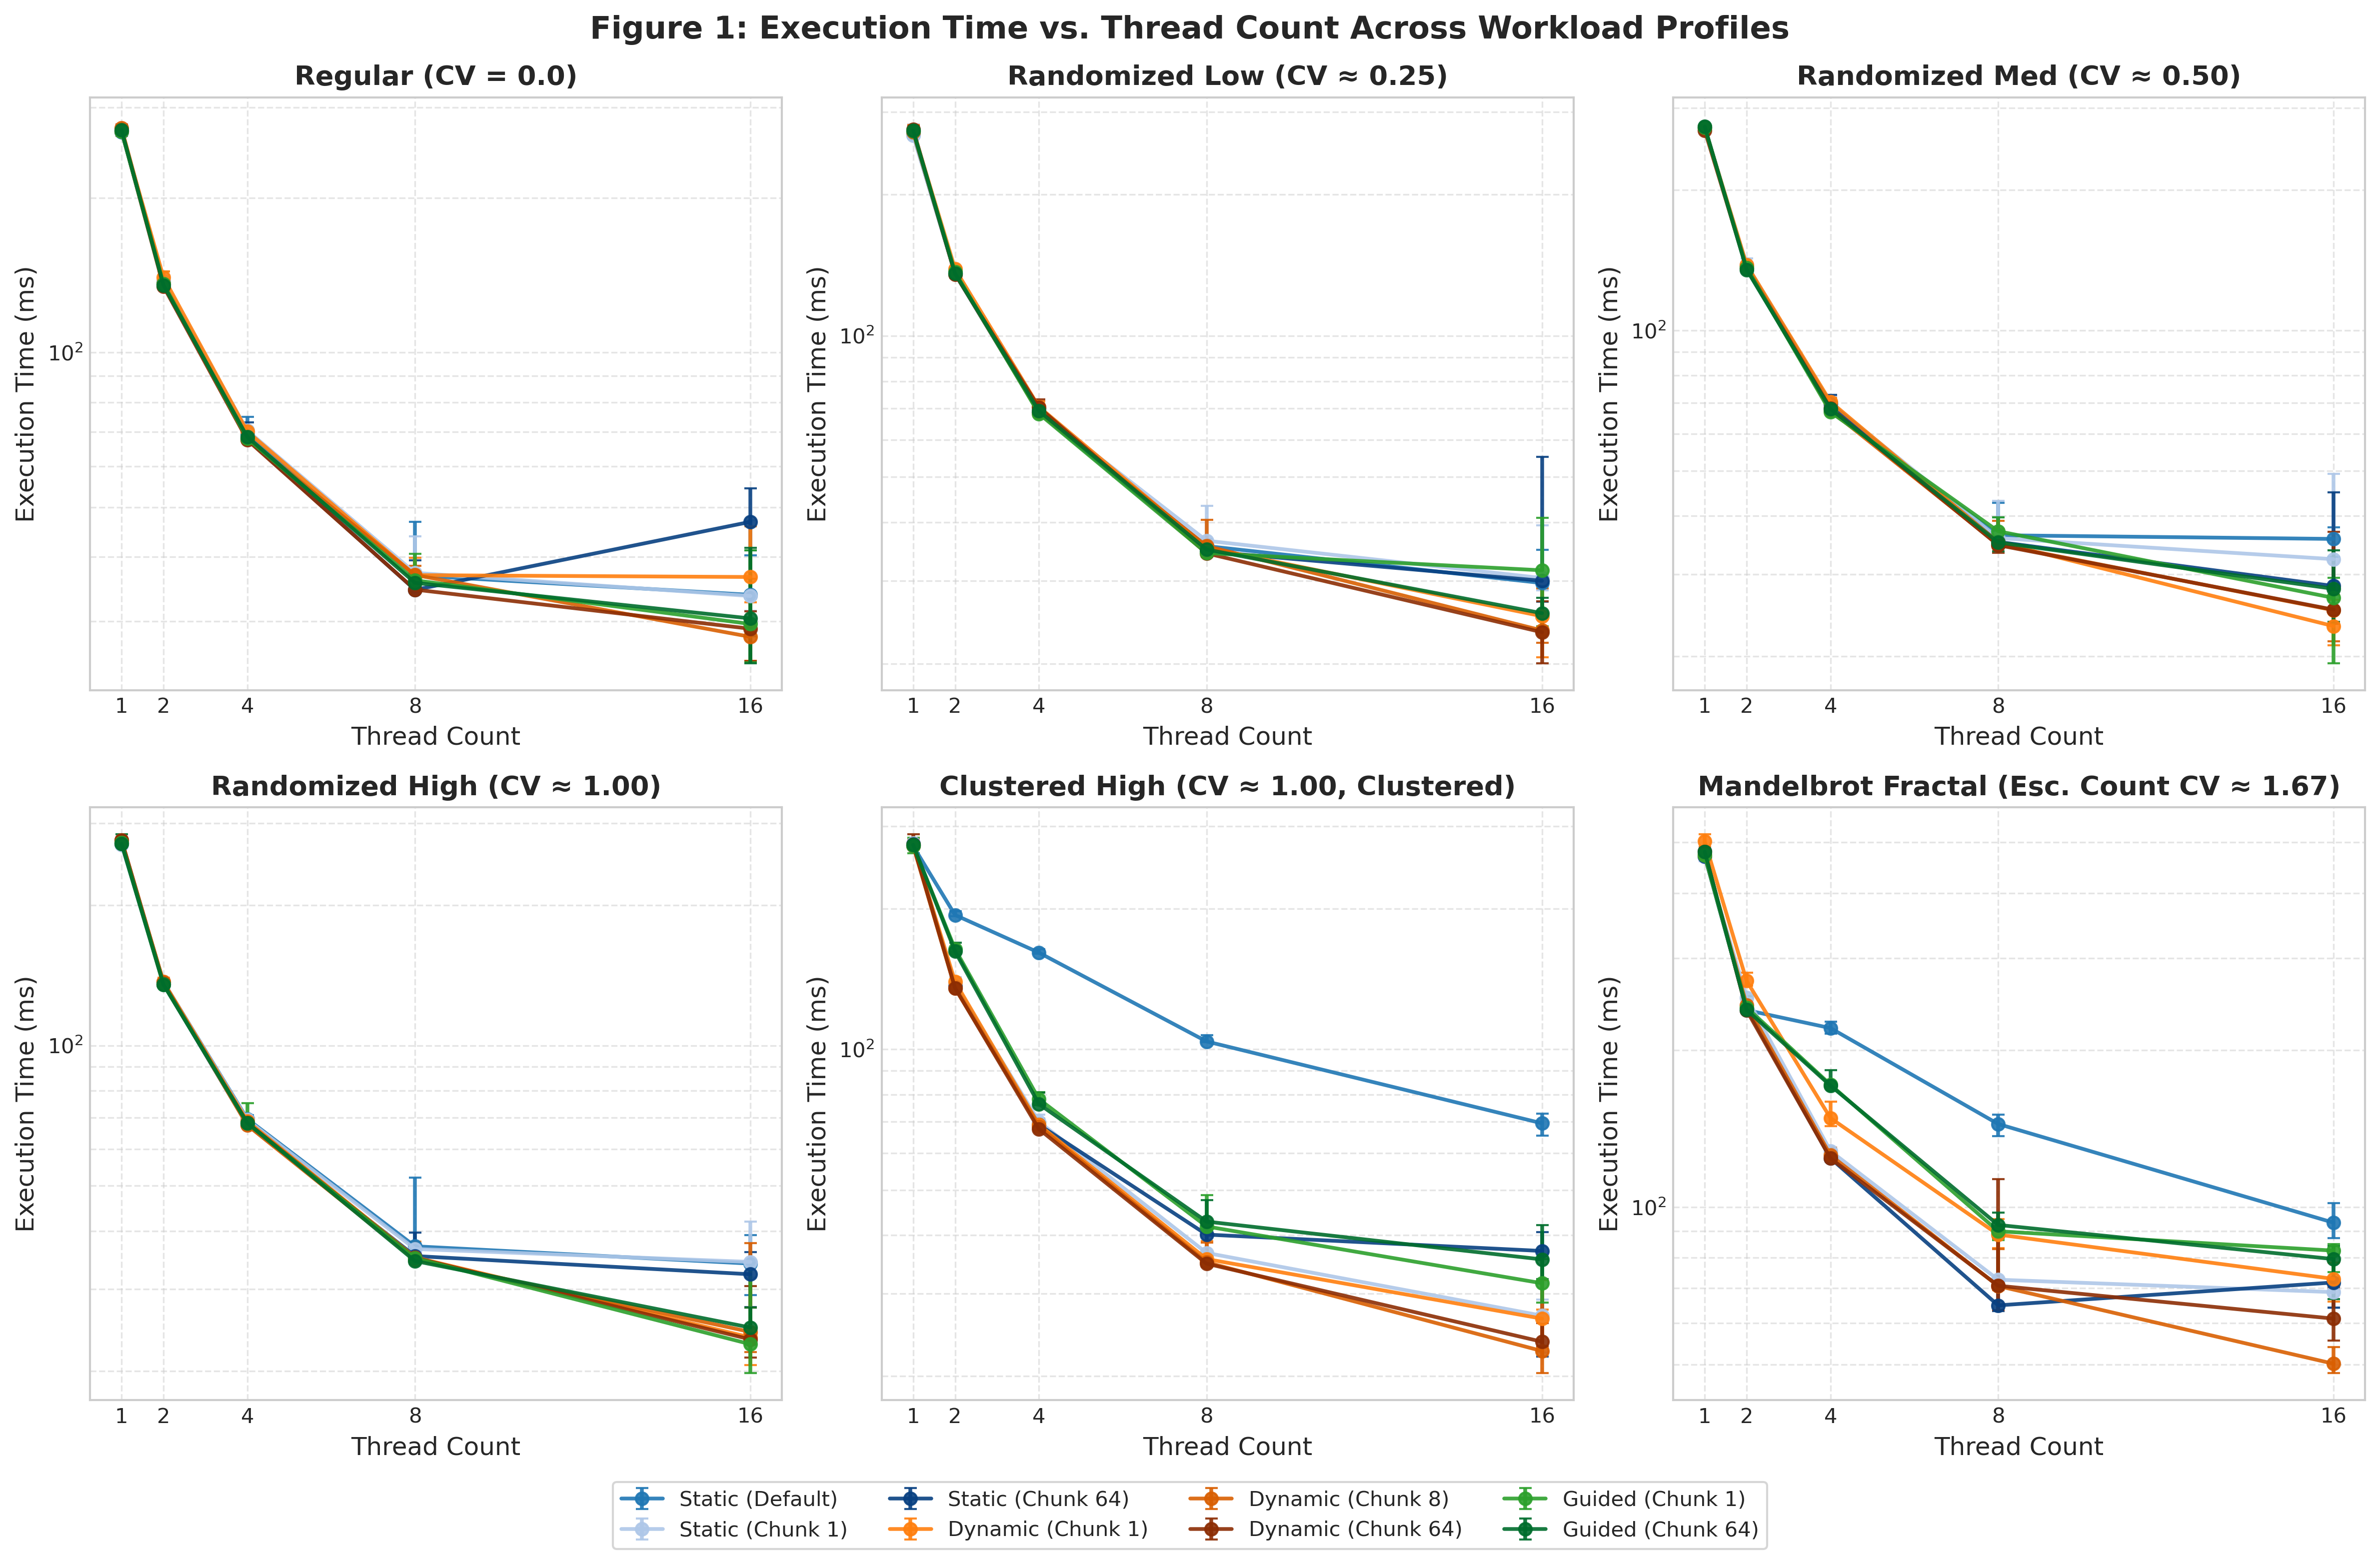
\includegraphics[width=\columnwidth]{figures/png/fig1_execution_time_vs_threads.png}
\end{figure}

\subsection{Hypothesis Evaluation}

\textbf{H1. static on regular workloads}

on regular 16 threads workload, static\_default median runtime = 33.75ms ($S_p=8.07x$ $E_p=50.4\%$). Not fastest, but in statistical noise of best static. And more importantly, on the same workload, dynamic\_c1 degrades to 36.55ms (8.3\% slower). So we support H1.

\textbf{H2. dynamic on irregular workloads}

on random high(est) irregularity (CV=1.00) we get +31.2\% on dynamic\_c64 and +32.8\% on guided\_c1 improvement wrt to static default. But also monotonic trend, with more irregularity more improvement. (on random low (CV=0.25) +20.8\% we get on dynamic scheduling) and (on clustered high (CV=1.00, worst for static) +67.4\% we get on dynamic\_c8) So we really support H2.

\begin{figure}[htbp]
\centering
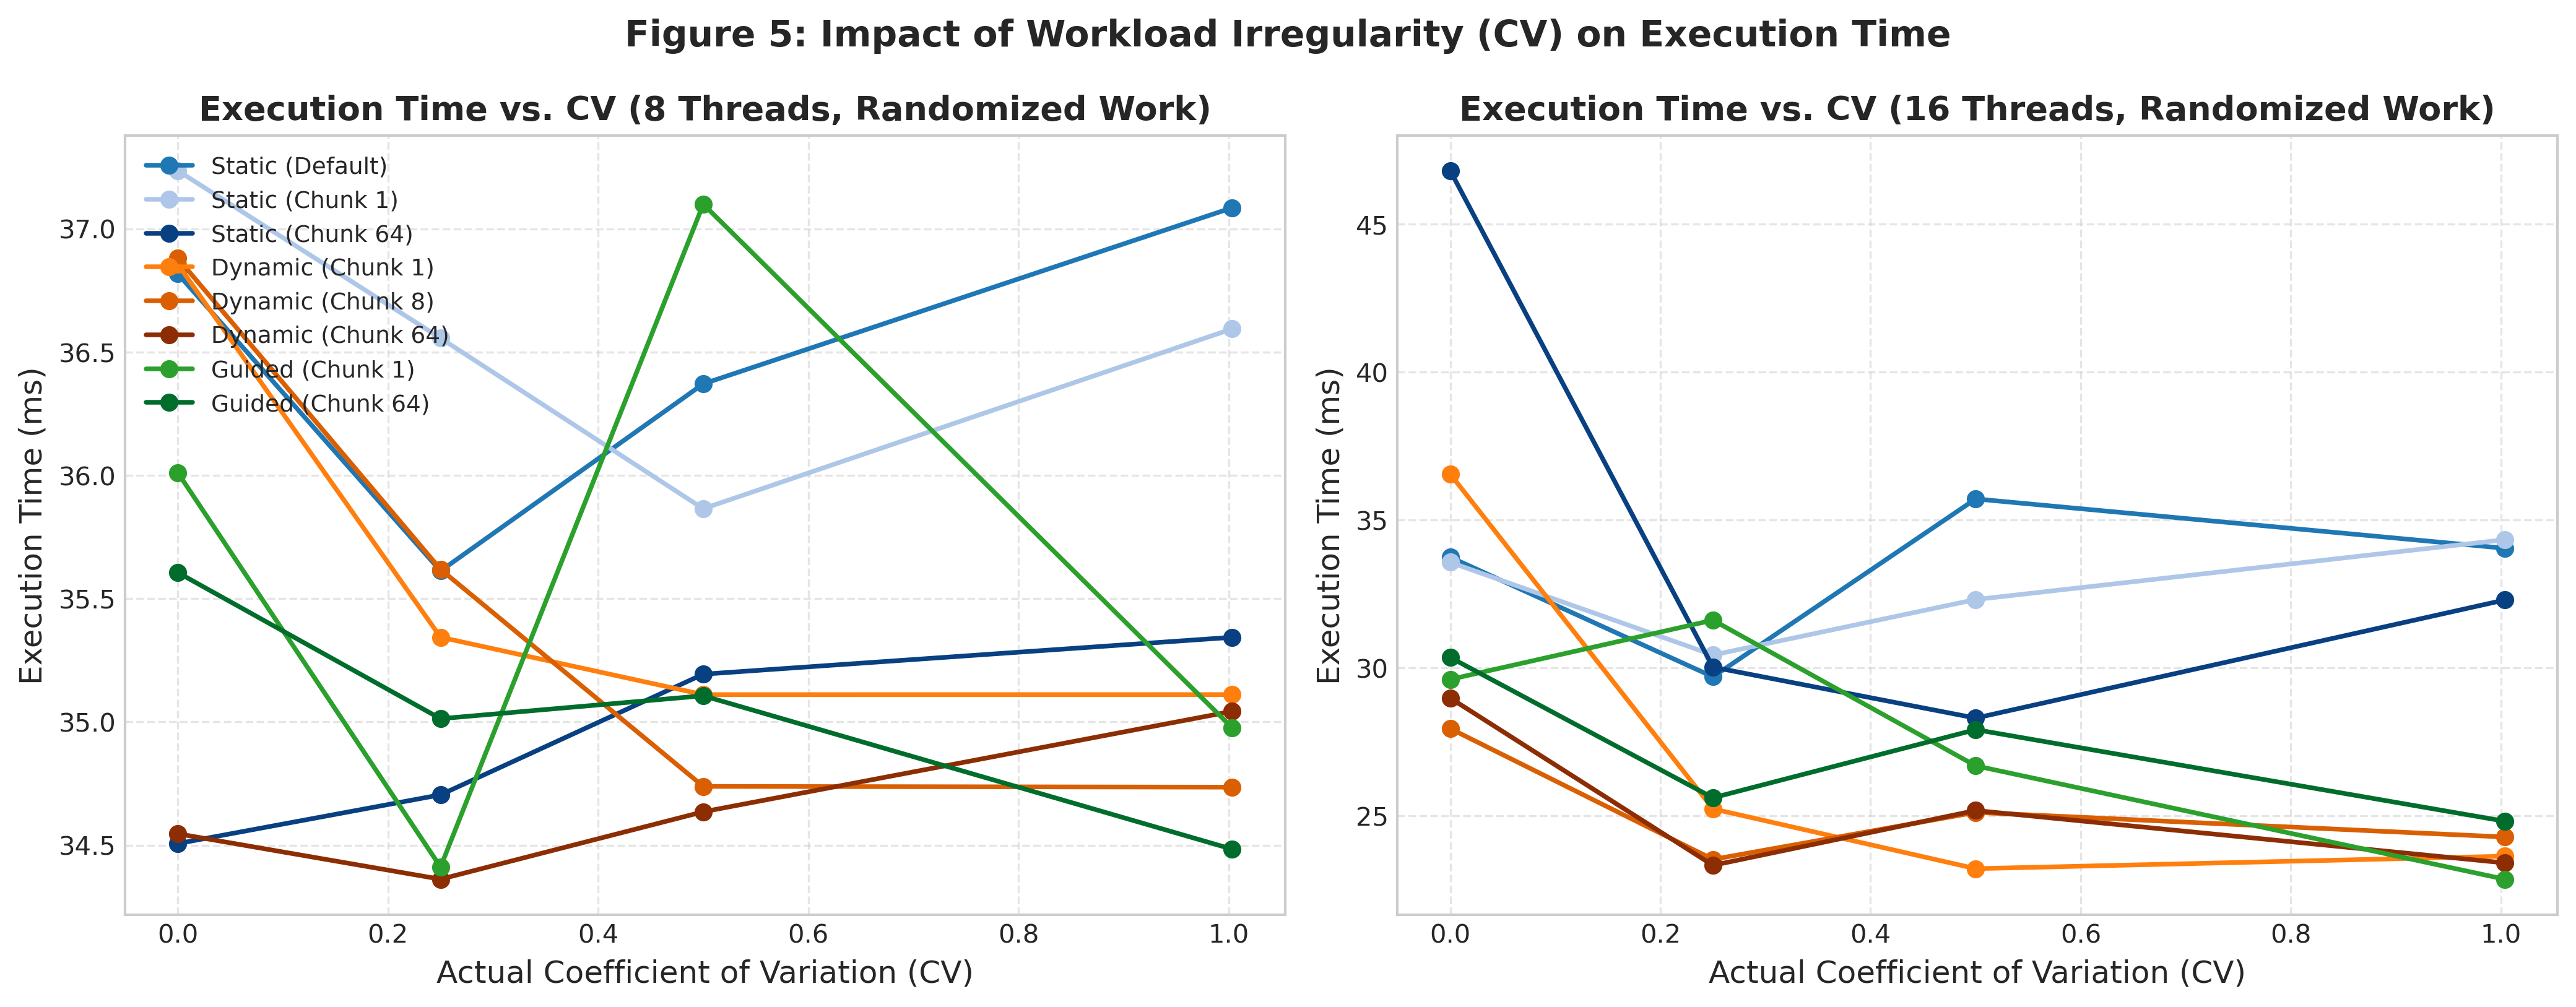
\includegraphics[width=\columnwidth]{figures/png/fig5_runtime_vs_workload_cv.png}
\end{figure}

\textbf{H3. Trade-off for guided scheduling}

Most improvement of guided scheduling is seen in random\_high. The performance of the guided\_c1 is the lowest median of all runs for all benchmarks (22.86 ms, $S_p=12.10\times$). But for the Mandelbrot benchmark with large chunks of non-escaping pixels near the boundary of the set, the speed of guided\_c1 is only 82.58 ms, much slower than dynamic\_c8 (50).

\subsubsection{H4. Spatial Organization vs CV}

Most impressive, the difference between \texttt{random\_high} and \texttt{clustered\_high}, same $CV=1.0035$, the same total work 50000000 ops. the same serial timings (similar 273...277ms). the randomized profile running at \texttt{static\_default} (16) threads takes 34.05ms ($S_p=8.13x$). the clustered one takes 69.43ms ($S_p=3.93x$). static scheduling breaks the job into contiguous chunks $\lceil N/P\rceil \sim 6250$ iterations per thread. For the clustered profile the 8 threads assigned to the range of indices $[N/4, 3N/4)$ collect almost all of the costly iterations. outer threads are just sleeping at the barrier.

For \texttt{dynamic\_c8} it is almost the same 24.29 (randomized) and 22.60 (clustered).

H4: for sure proven. CV is not enough to predict load imbal. space-autocorr of iter. costs is also important.

\begin{figure}[htbp]
\centering
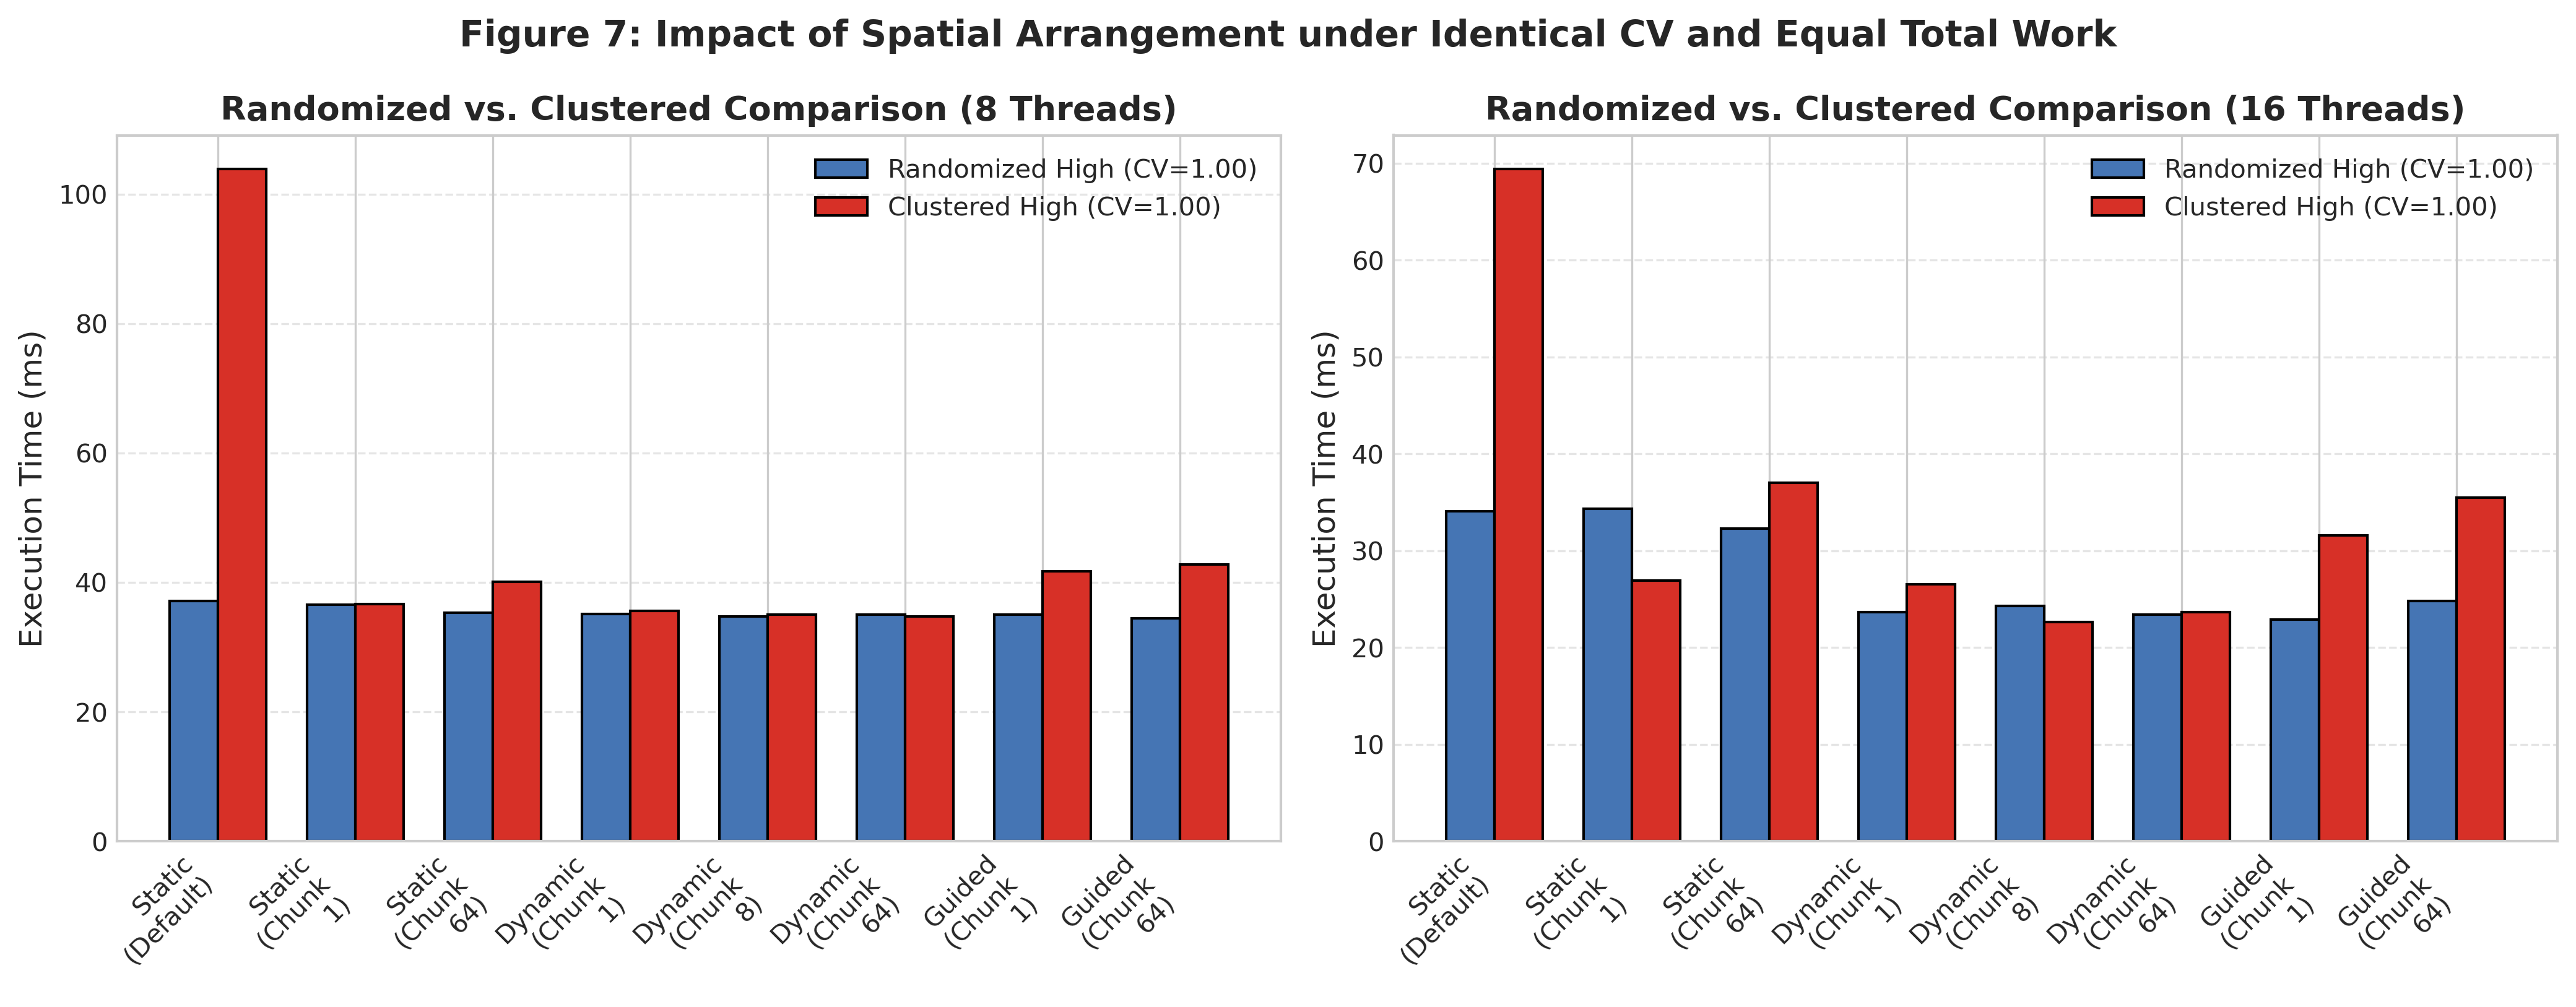
\includegraphics[width=\columnwidth]{figures/png/fig7_spatial_clustering_comparison.png}
\end{figure}

\subsubsection{H5. Chunk Size and Contention}

We have confirmed via probe measurement that the dynamic scheduling based on unit-chunk comes with significantly higher coordination overhead. In 16 thread, the probe execution time of \texttt{dynamic\_c1} is 2.75ms while that of \texttt{dynamic\_c64} is 0.32ms, and the ratio of overhead is 8.6 times. The 2.75ms dispatch overhead forms a significant portion of total time if we have small work per iteration (like normal loop with $W_{\text{base}}=500$), hence a regression is noticed in H1. For the irregular workloads with dominant load imbalance, the story is different, with 2.75ms of dispatch cost, \texttt{dynamic\_c1} on the cluster workload shows 26.52ms, while static default shows 69.43ms. There is a 61.8\% improvement. So hypothesis H5 is strongly supported.

\begin{figure}[htbp]
\centering
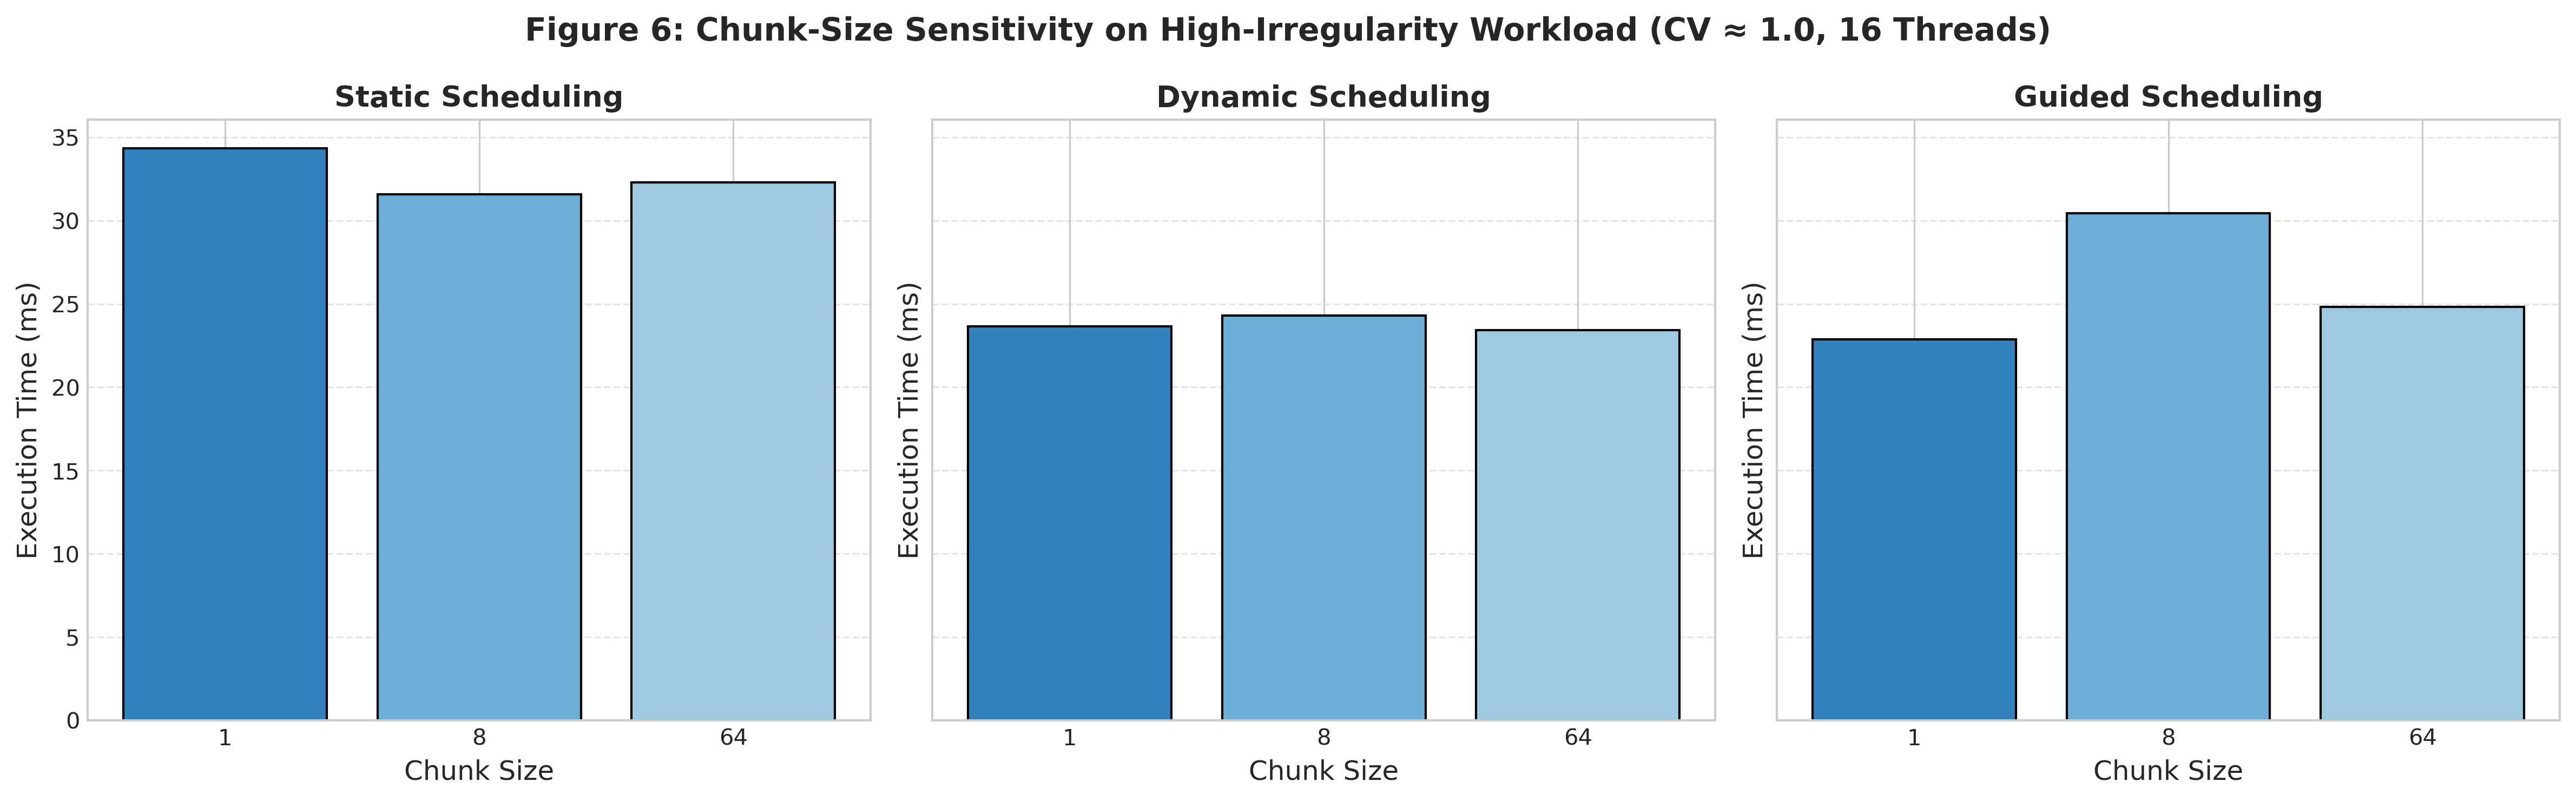
\includegraphics[width=\columnwidth]{figures/png/fig6_chunk_size_sensitivity.png}
\end{figure}

\subsection{Scaling Behaviour and Parallel Efficiency}

Figure \ref{fig:arch} gives a summary of key scaling points. For all irregular workloads, the parallel speed-up with dynamic/guided scheduling is nearly linear up to 8 physical cores. A speed-up of $S_p \approx 6.8$--$7.9\times$ is observed at $P = 8$. Enabling the second SMT thread per core at $P = 16$ brings an additional $\approx 60\%$ in the speedup increment, for the irregular cases. ($S_p = 12.10x$ best). The synthetic kernel is ALU bounded (for integers) and very low in memory pressure. This creates conditions where SMT can make use of otherwise dormant execution resources of a stalled pipeline. The parallel efficiency ranges from 75.6\% (\texttt{guided\_c1} on random high) down to 24.6\% (\texttt{static\_default} on clustered high) at $P = 16$, which is a near complete collapse of load imbalance.

For the static default case on clustered workload, the efficiency monotonically deteriorates with $P$ increasing beyonds when the central cluster no longer covers the thread count. This is due to a mismatch in space between the bounds of static assignment and the clustering of expensive iterations. For the same workload, the dynamic scheduling keeps the efficiency above 60\% for the full range of threads.

\begin{figure}[htbp]
\centering
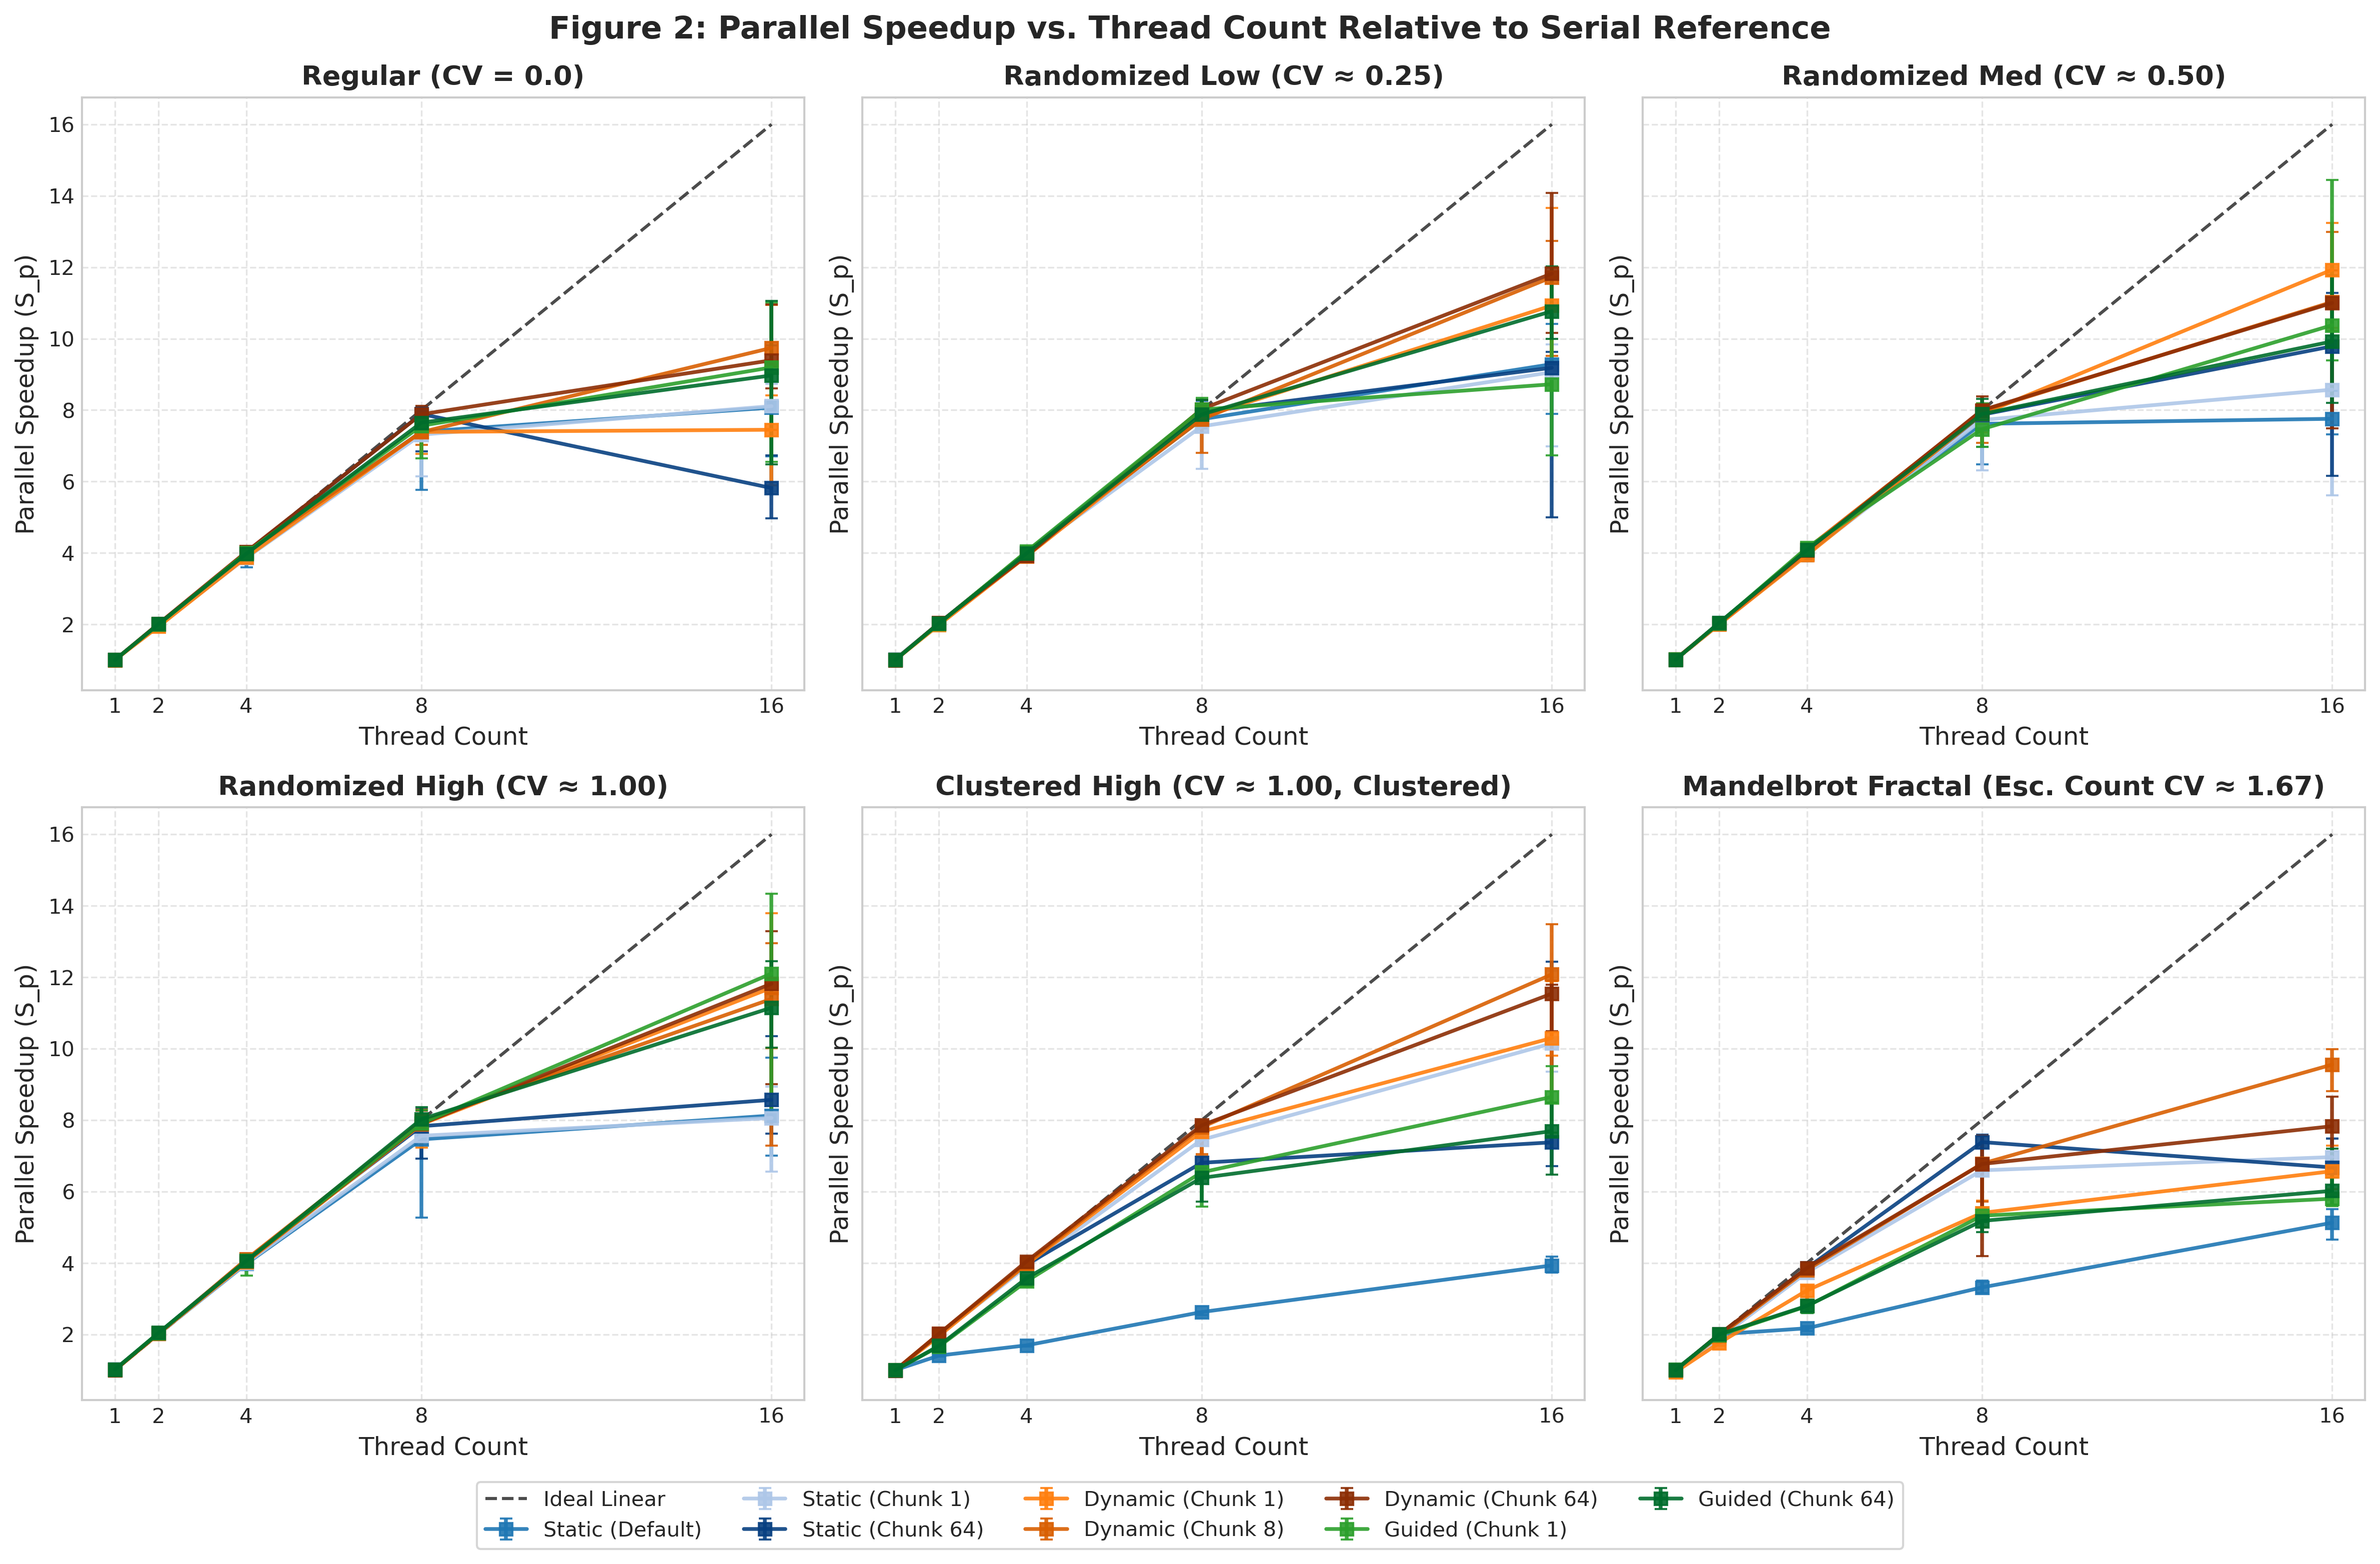
\includegraphics[width=\columnwidth]{figures/png/fig2_speedup_vs_threads.png}
\end{figure}

\begin{figure}[htbp]
\centering
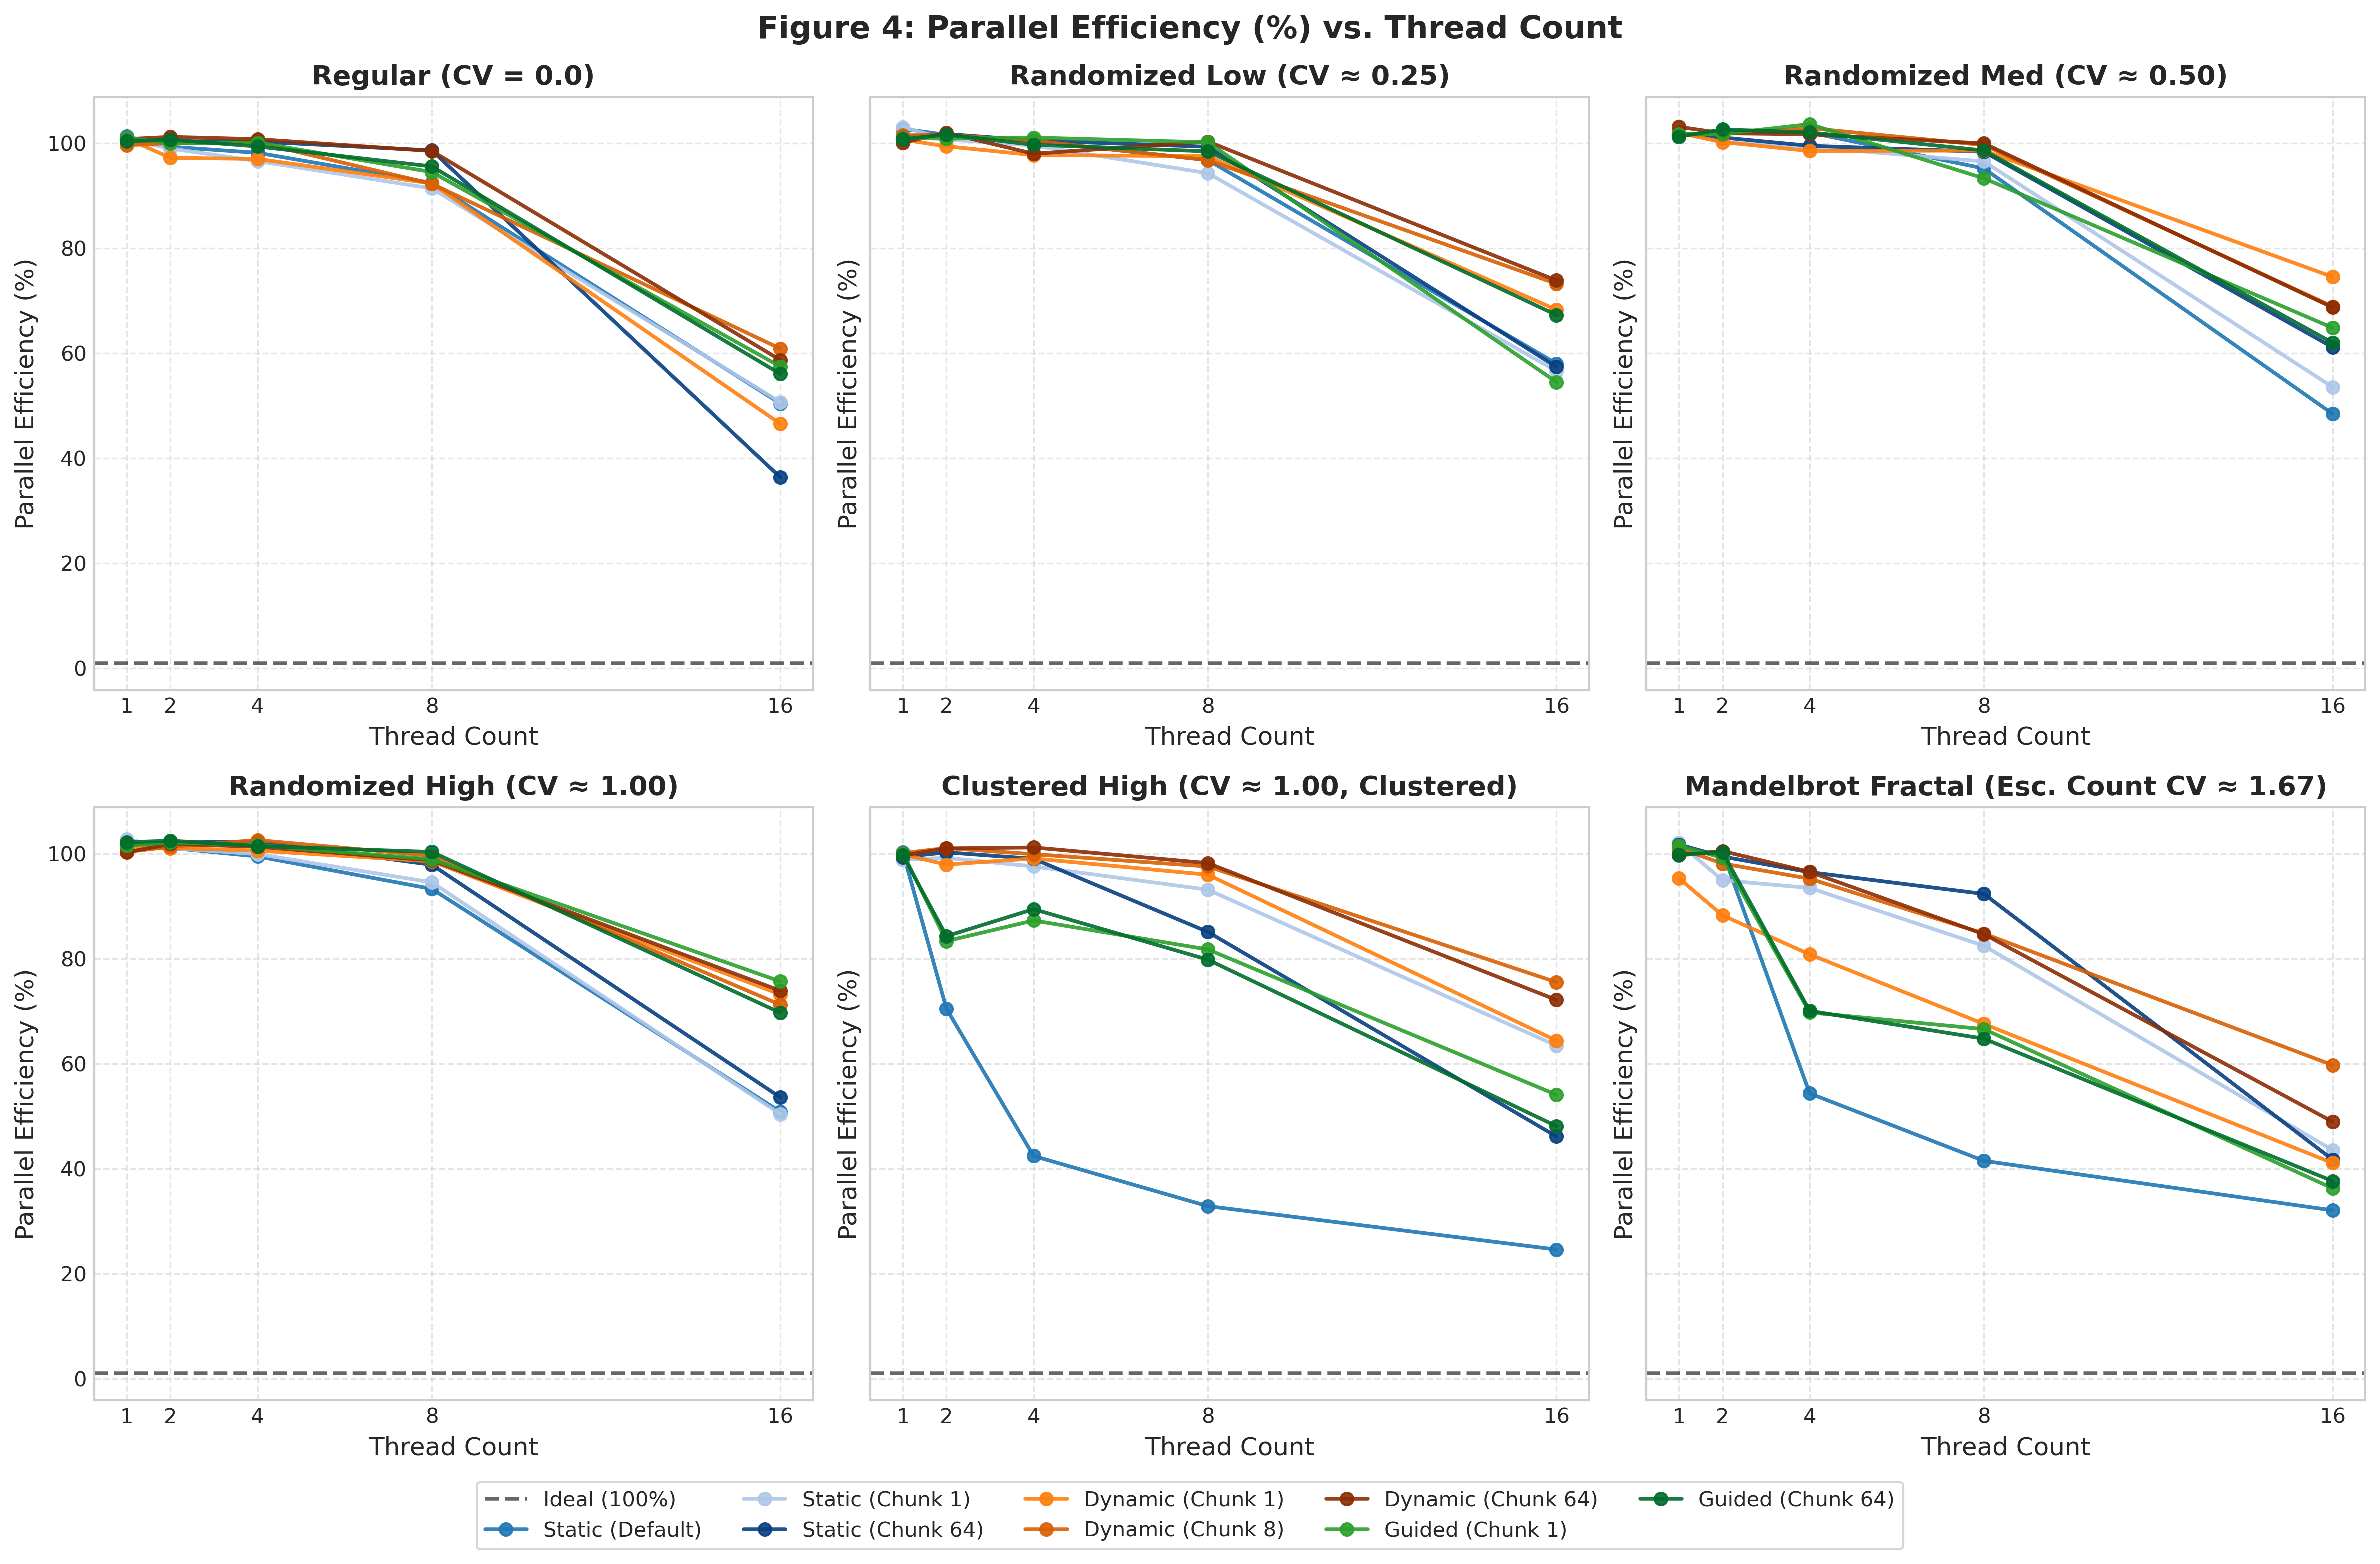
\includegraphics[width=\columnwidth]{figures/png/fig4_efficiency_vs_threads.png}
\end{figure}

\subsection{Dispatch Overhead vs. Chunk Size}

Table \ref{tab:overhead} Probe-measurement of overhead of the relationship of chunk size ($C$) and coordination overhead at 16 threads. This is roughly $1/C$, as predicted by the theory: number of atomic aquisitions of workqueue ($N/C$) per thread.

\begin{table}[htbp]
\centering
\caption{Low-work dispatch overhead @ 16 threads}
\label{tab:overhead}
\begin{tabular}{llr}
\toprule
\textbf{Policy} & \textbf{C} & \textbf{Probe-Time (ms)} \\
\midrule
\texttt{static\_default} & --- & 0.18 \\
\texttt{static} & 1 & 0.18 \\
\texttt{static} & 64 & 0.09 \\
\texttt{dynamic} & 1 & 2.75 \\
\texttt{dynamic} & 8 & 0.72 \\
\texttt{dynamic} & 64 & 0.32 \\
\texttt{guided} & 1 & 0.43 \\
\texttt{guided} & 8 & 0.10 \\
\bottomrule
\end{tabular}
\end{table}

The overhead of dispatching under static scheduling is practically independent of C, since for cyclic static the chunk boundaries are pre-computed without any atomic ops. Under dynamic scheduling $C=1$, there are $N=100k$ atomics to do per $P=16$ threads (say $\sim 6.25k$ per thread), which dominates the cost for this granularity.

\subsection{Mandelbrot Validation}

\begin{table}[htbp]
\centering
\caption{Mandelbrot Bench (1200x900 400 max) @ 16 threads}
\label{tab:mandel}
\begin{tabular}{llrrl}
\toprule
\textbf{Policy} & \textbf{C} & $\tilde{T}$ (ms) & $S_p$ & $\Delta T_{\text{rel}}$ \\
\midrule
Serial & --- & 479.0 & $1.00x$ & (---) \\
\texttt{static\_default} & --- & 93.41 & $5.13x$ & (Baseline) \\
\texttt{static\_c1} & 1 & 68.76 & $6.97x$ & (+26.4\%) \\
\texttt{dynamic\_c1} & 1 & 72.90 & $6.57x$ & (+22.0\%) \\
\texttt{dynamic\_c8} & 8 & 50.13 & $9.55x$ & (+46.3\%) \\
\texttt{dynamic\_c64} & 64 & 61.18 & $7.83x$ & (+34.5\%) \\
\texttt{guided\_c1} & 1 & 82.58 & $5.80x$ & +11.6\% \\
\texttt{guided\_c8} & 8 & 80.97 & $5.92x$ & +13.3\% \\
\bottomrule
\end{tabular}
\end{table}

Detailed Mandelbrot results table \texttt{tab:mandel}. \texttt{dynamic\_c8} gets best speedup $9.55x$ with 59.7\% eff. Row by row mapping of mandelbrot pixels to 1d iteration space makes rows near real axis (bulb + cardioid border pixels) much more expensive than top/bottom rows of frame. Thread assigns consecutive rows bands in static default which makes unevenness with number of threads (another kind of spatial clustering similar to constructed profile of \texttt{clustered\_high}).

Notice a relative low performance of guided scheduling in this scenario compared to synthetic random-high load. Guided with reduced chunk sizes for random-high (evenly spreaded costly iterations) makes each thread getting mix of cheap and expensive work bit by bit and smoothes the load. Mandelbrot on the other hand makes high concentrated by space in rows so big initial chunks of guided are getting lot of expensive pixels at once and last part of benefit from shrinking chunk sizes (at the end) is reduced since tail rows that get late are comparatively cheap.

\begin{figure}[htbp]
\centering
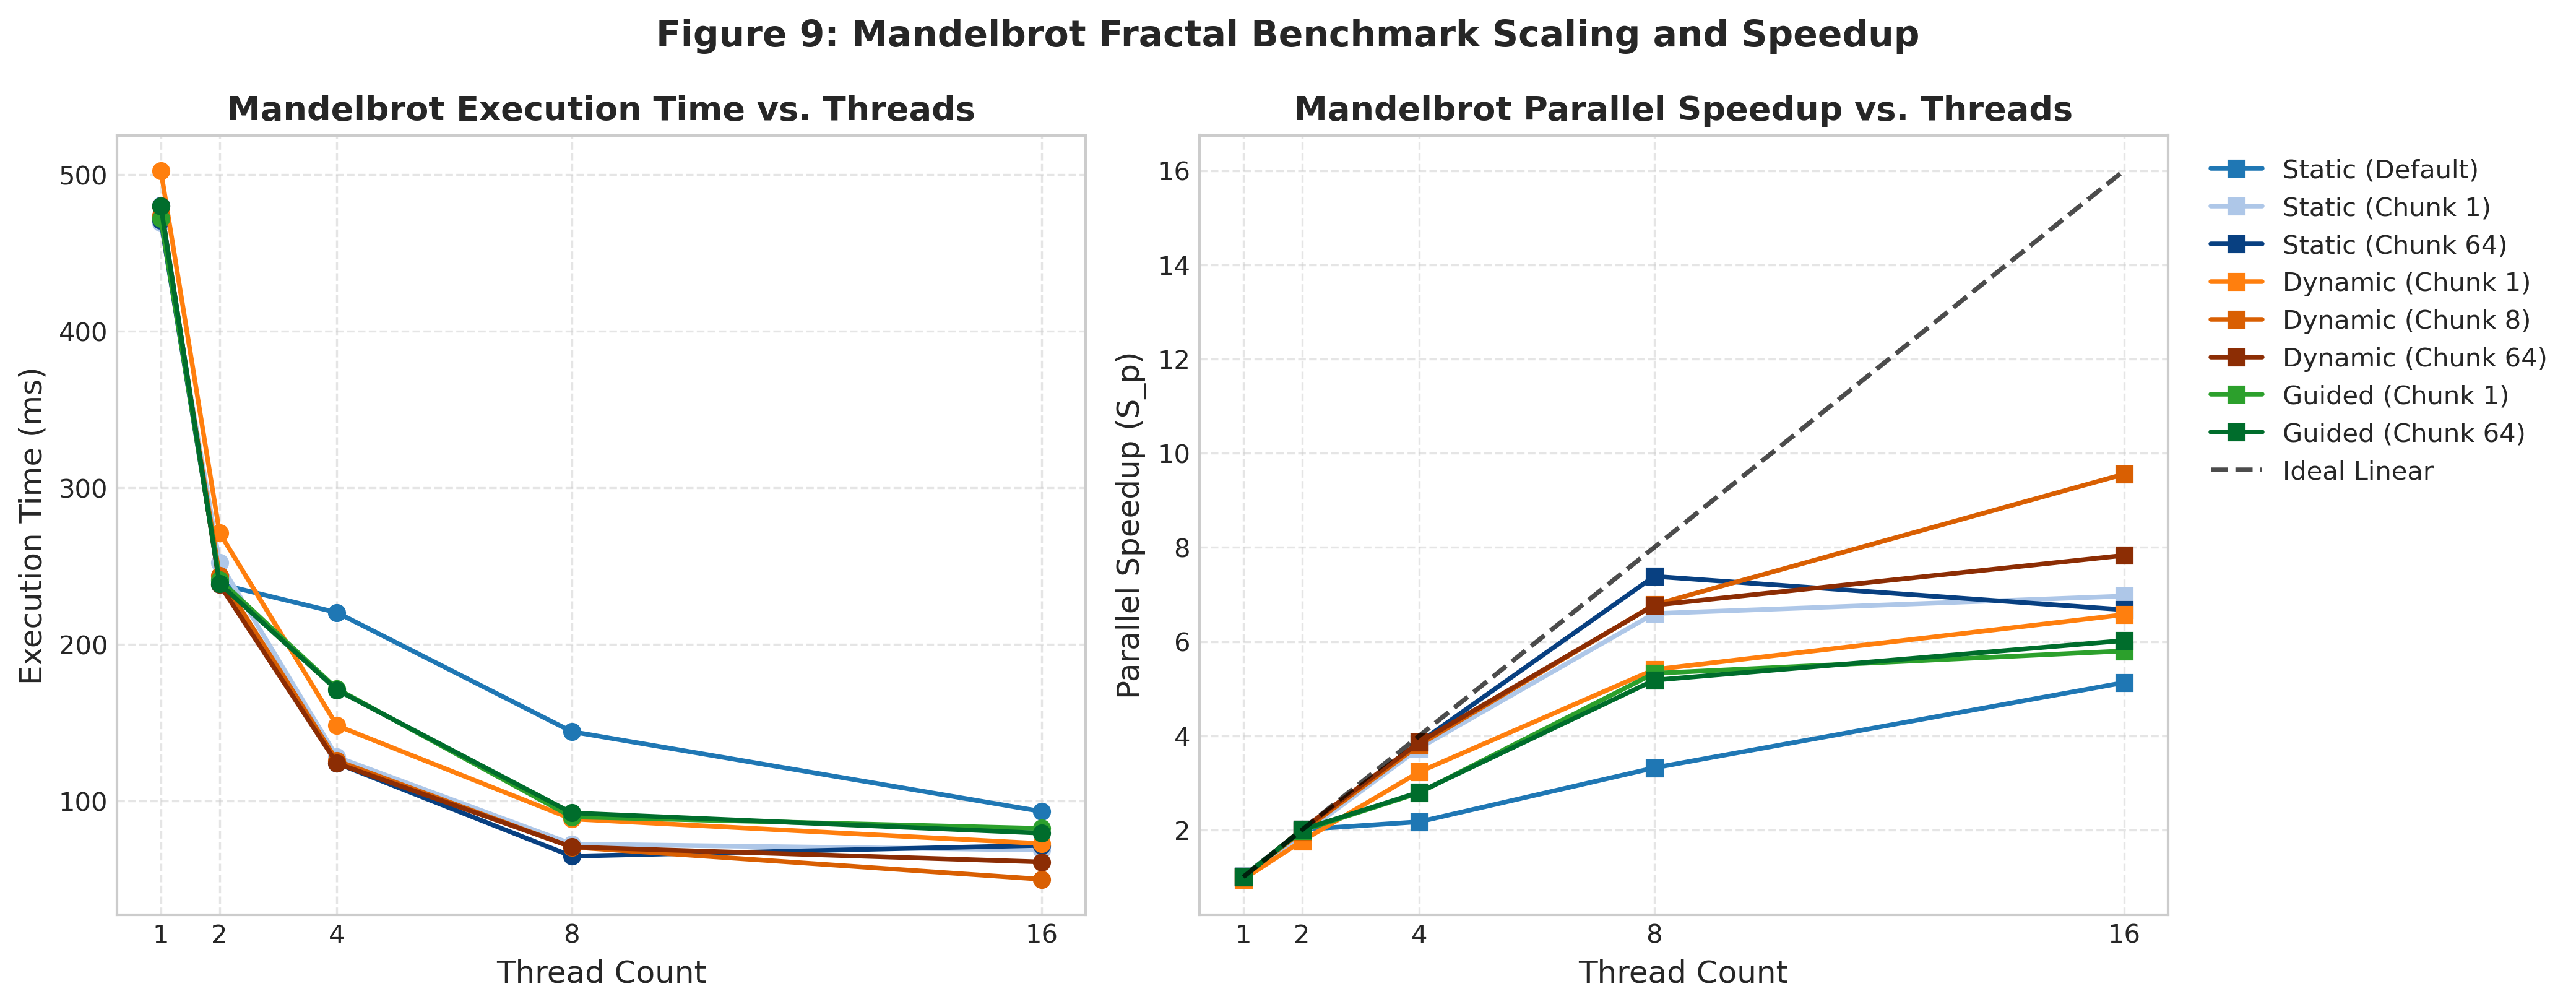
\includegraphics[width=\columnwidth]{figures/png/fig9_mandelbrot_results.png}
\end{figure}

% -------------------------------------------------------
\section{Discussion}

\subsection{Spatial Arrangement Result}

This result is the most practically interesting one. It means that two workloads with the same CV, the same total work, and the same serial runtime, can have different 2+ performance of parallelisation in static scheduling by more than a factor of 2. This happens because of the static assignment $\lceil N/P \rceil$ block size: a large cluster of expensive iterations, which fits in a contiguous portion of space and overlaps with a subset of thread assignments, makes some threads become stragglers while other threads wait for them at the synchronisation barrier. CV measures the marginal distribution of the cost of the iterations but omits their joint spatial distribution. A full performance model would have to include the spatial autocorrelation of $W$ in the index of iterations. This is not a metric that is available from standard descriptions of workloads.

\begin{figure}[htbp]
\centering
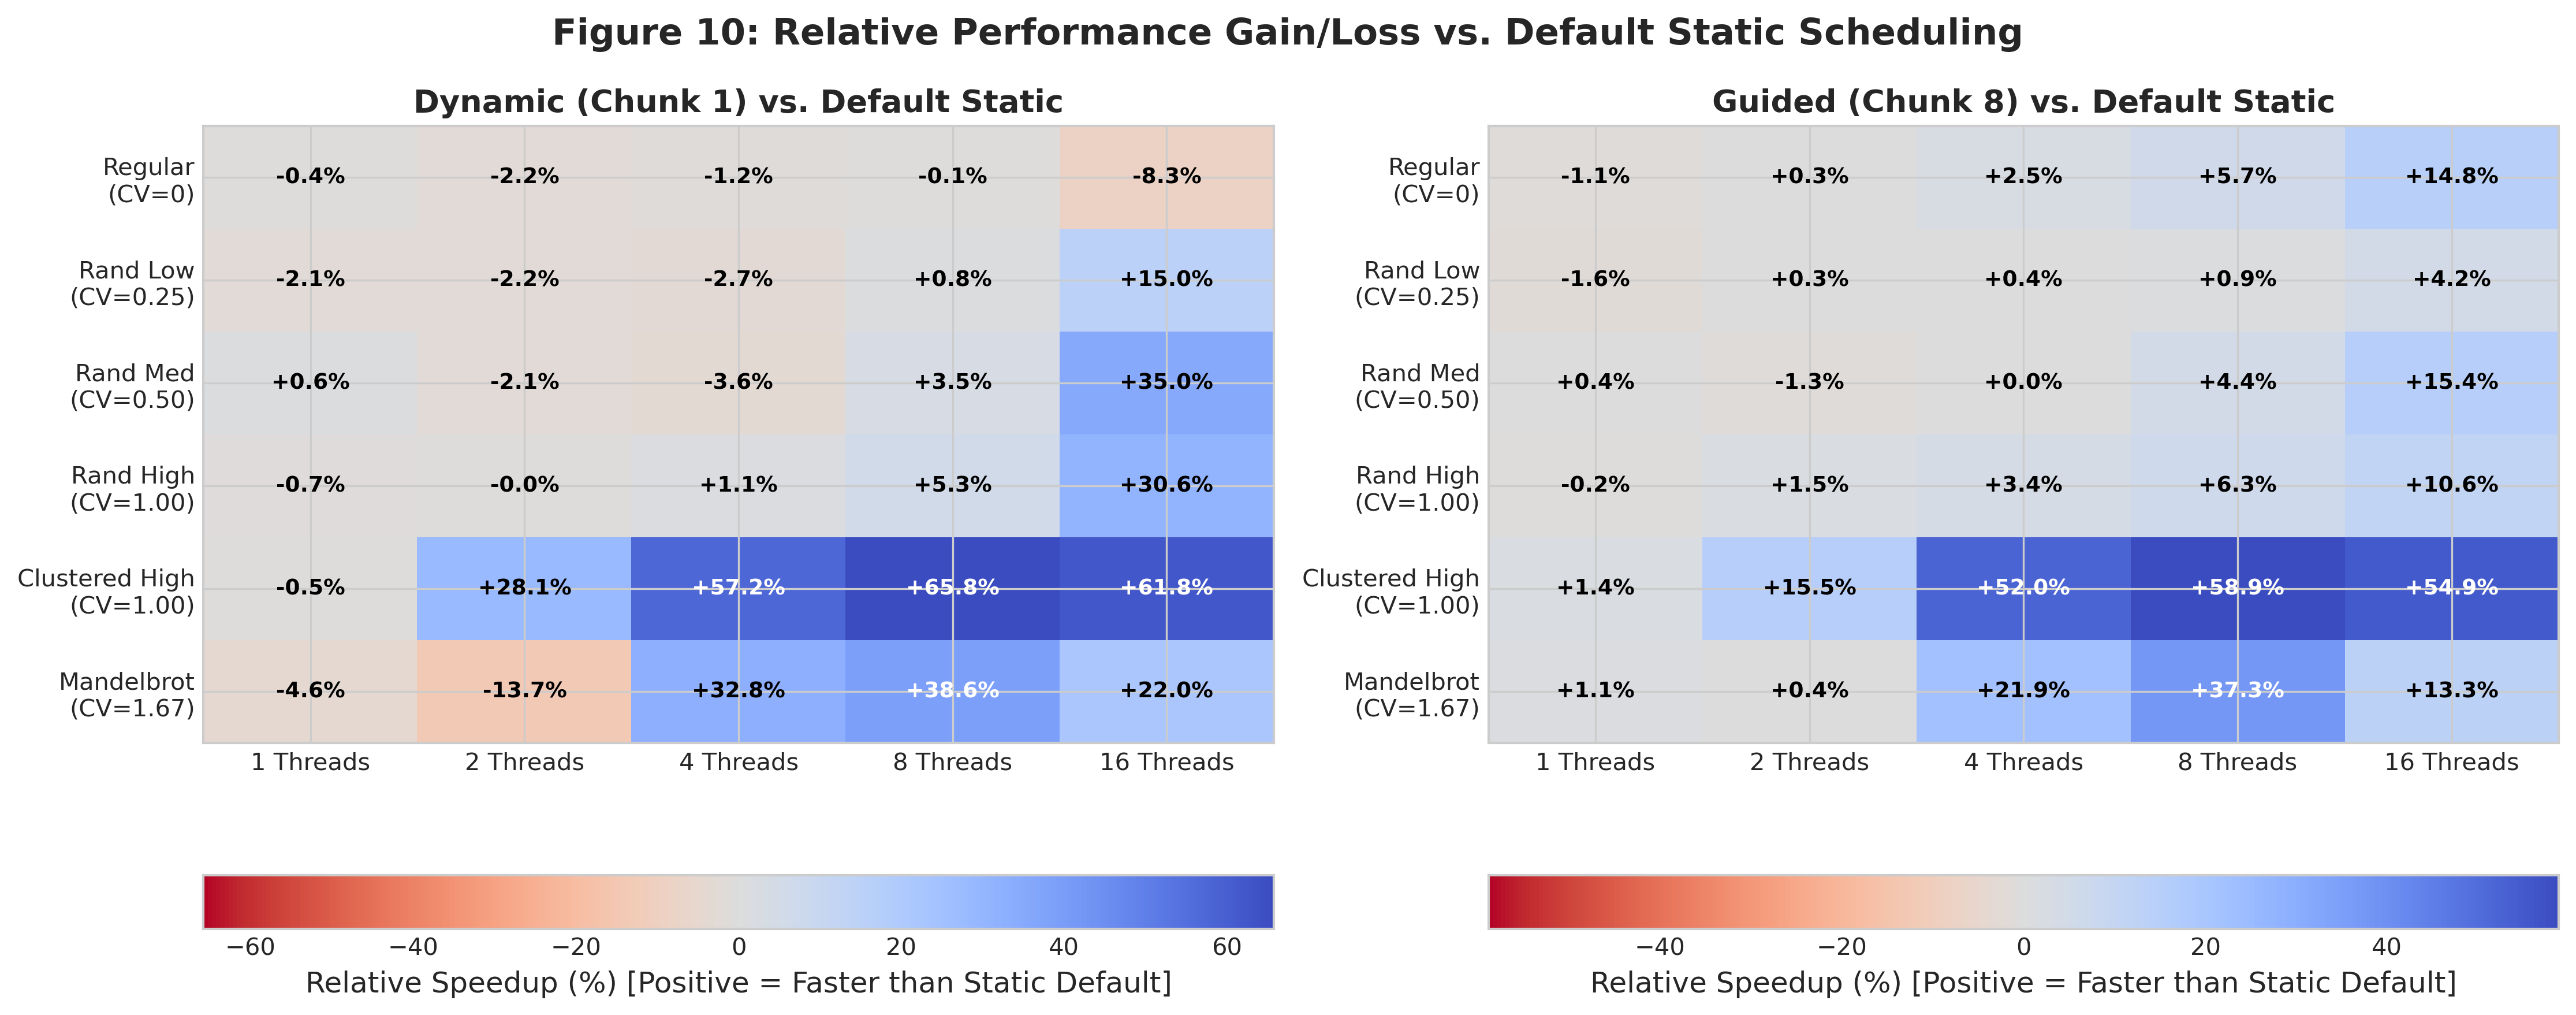
\includegraphics[width=\columnwidth]{figures/png/fig10_relative_performance_heatmap.png}
\end{figure}

This has practical consequences for adaptive parallelisation: Any cost predictor that uses only heuristics about the input size, without profiling the spatial distribution of work, is going to mis-classify the type of clustered-irregular loops as if it were randomised-irregular and may recommend to use static when a dynamic approach would be needed.

\subsection{Why Dynamic C=8 dominates all profiles}

\begin{figure}[htbp]
\centering
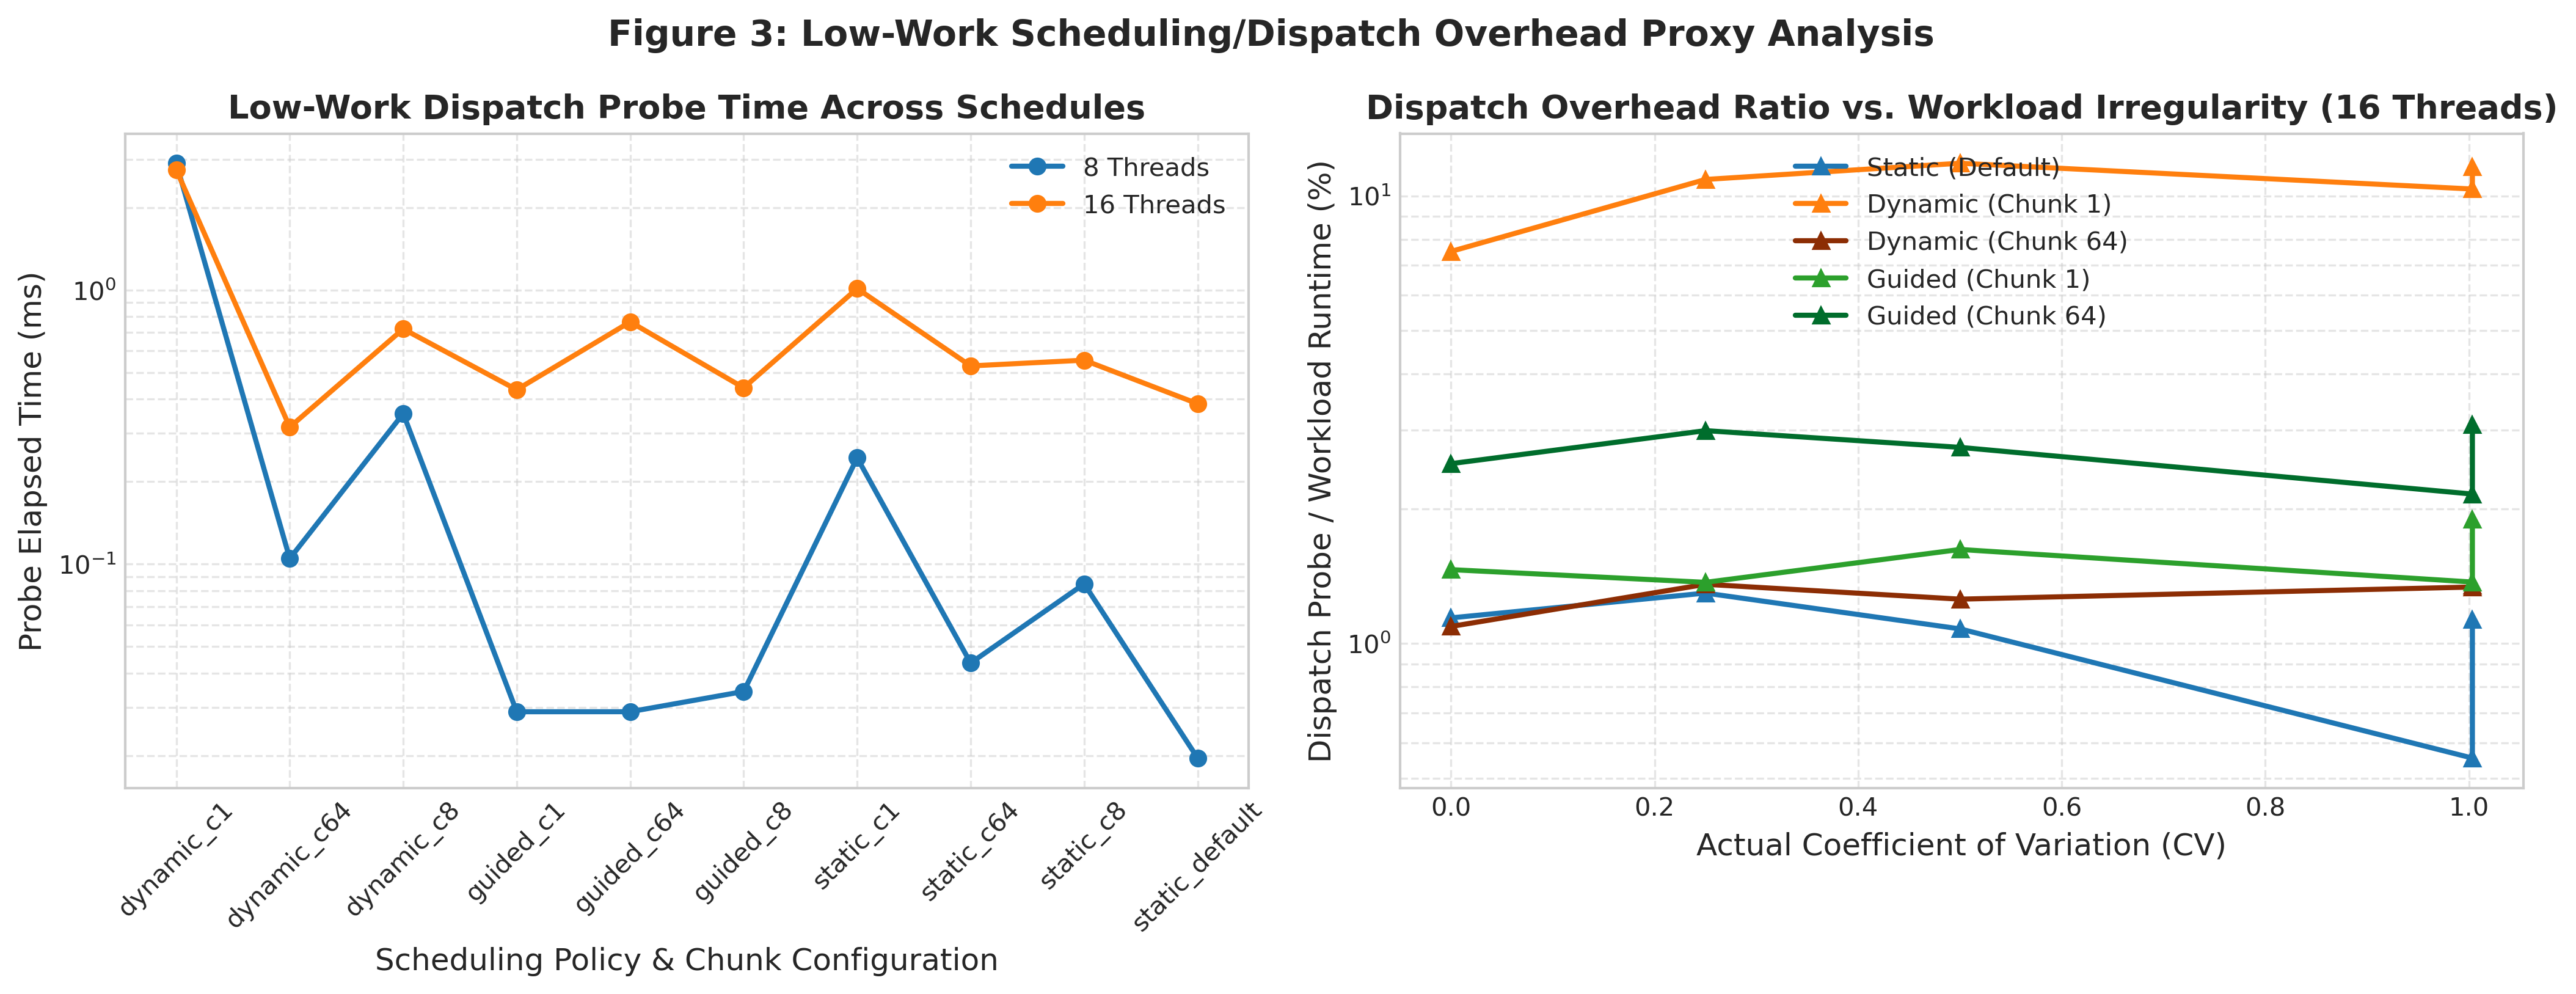
\includegraphics[width=\columnwidth]{figures/png/fig3_scheduling_overhead_vs_irregularity.png}
\end{figure}

Why Dynamic C=8 dominates all profiles?

One of the impressive things about the reliability of dynamic\_c8 on the fake irregular and mandelbrot benchmarks is that it indicates a sweet spot where the trade-off between costs is favourable. So, at C=1 atomic queue contention is dominating (for 100k-iteration loops with 16 threads). And at C=64 tail stragglers are getting significant, i.e. last thread grabs a 64-iteration chunk that happens to be from the expensive central area, then the other threads have to wait 64-iterations of work at the barrier (at $W_{\text{base}}=500$ about $3.2 \times 10^4$ hash operations). For C=8 that is 1/8th of the straggler effect as compared to C=64 but only 1/8x less queue ops than at C=1.

That's consistent with the theory in \cite{hummel1992factoring} that the optimal chunk size is $O(\sqrt{N / (P*\text{dispatch-overhead-per-chunk})})$. For these parameters, the answer is single-digit to low double digit values.

\subsection{SMT Scaling \& Regular Workload Weirdness}

An interesting finding on regular work is that although static\_default doesn't have any dispatch overhead, dynamic\_c8/guided\_c8 win by 17-15\% at 16 threads vs static\_default, which is not a load imbalance effect (all iterations have exactly the same cost) but rather the cyclic-round-robin way iterations are assigned across threads in chunked static and runtime-dispatched policies can be a more scattered way of assigning iterations across threads (and may even help with cache line utilisation/false sharing of output buffer relative to the monolithic block assignement in static\_default).

Or it can lead to a different code path internally in libgomp which is less synchronisation heavy at the start/end of parallel region under SMT if we take the schedule(runtime) path, which is not expected a priori and we need to dig further with hwcounters.

\subsection{Limitations of the Dispatch Probe}

This is the conservative lower bound from a probe approach, but you cannot directly subtract it from workload execution time to get "pure computation". Because under high ALU load, it will be the thread fighting over execution units/cache bandwidth for a different sort of contention (vs near idle probe threads). So probe time is the floor estimate of the overhead. You'll likely have higher overhead of the actual experience inside a workload loop, due to interference. We do explicitly mark all the probes as proxys in the analysis pipeline and figures.

\subsection{Generalisability}

(single socket 8core moblie APU under wsl2). So with multi-socket numa you'll have additional remote memory latency for shared dynamic work queue, which likely blows up the overhead for fine-grained dynamic scheduling (more than we see here). for intel hybrid asymmetric clocks (p-cores and e-cores) there would be a fundamentally different lbe problem, because static scheduling doesn't match work amounts to core throughput. and with server class amd epyc (64-192) cores, the atomic contention for dynamic\_c1 would blow up significantly favoring larger chunk sizes.

\section{Limitations and Future Work}

\subsection{Current Limitations}

\textbf{Same arch:} everything ran on AMD Ryzen 7 6800H (Zen 3+, single NUMA domain). We know that overhead of dynamic vs. static scheduling is roughly proportional to threads/memory topology, and break-even CV (where dynamic scheduling becomes beneficial) could change on multiple-socket machines.

\textbf{Range of C is small:} $C \in \{1, 8, 64\}$ was explored; performance of $C \in \{2, 4, 16, 32, 128, 256\}$ is uncharted. From our probing, there seems to be roughly inverse relation between C and overhead, but finer sampling is needed to get exact curvature in C$\rightarrow$performance space.

\textbf{Static N:} $N=100,000$ is used in synthetic benchmark. For loops with N in millions (common for stencils, molecular dynamics, etc.) there could be different operating points for chunk efficiency; also, larger C (more aggressive amortisation of dispatch overhead) could be beneficial.

\textbf{Synthetic nature of kernel:} our int hash kernel is ALU-bound, high-IPC, low-cache-pressure. In actual scientific codes, FPU ops, indirection, branch mispredictions, vectorisation, etc. are present, and these may have different interactions with loop scheduling.

\textbf{For GNU libgomp only.} The measuring for dispatch overheads is specific to GNU libgomp implementation. In case of LLVM libomp or Intel libiomp5 there are different internal synchronisation approach and overhead profile can be significantly different (especially for dynamic scheduling).

\subsection{Future work}

\textbf{Adaptive selector.} This study indicates that it may be beneficial to have a short pilot run that allows us to profile the spatial correlation of the iteration cost, so that an automated selector may decide between static and dynamic schemes. It would be logical to implement such an adaptive selector in the performance-portable abstraction layer.

\textbf{Task parallelism comparison.} Task based parallelism in OpenMP might give even more flexibility in scheduling than worksharing loops. It may be able to cope with tree like structures, or data-dependent irregular workloads that chunked loops might not. It would be useful to see a direct comparison under the same conditions to complement this work.

\textbf{Multi-socket and heterogeneous.} Repeat the factorial experiment on an AMD EPYC dual-socket machine, and on an Intel Alder Lake (P+E core) system to see if we do see a difference between CV and spatial or whether in high thread count, the NUMA-costs dominate the choice in the scheduling.

\textbf{Vectorisation interaction.} Chunked (both static and dynamic) might interact with auto-vectorisation, very small chunks might stop the compiler to produce SIMD code for the inner loop. It would be interesting to study this interaction with \texttt{-march=native} and the explicit \texttt{\#pragma omp simd} annotations, to see if there is a need to factor in vectorisation for selection of the scheduling policy.

\section{Conclusion}

This work reported a controlled empirical study of openmp loop scheduling for a full factor matrix of 2,492 execution records over an AMD Ryzen 7 6800H (8 phys 16 SMT) Zen 3+ processor. The key findings of the study validated and/or refined five directional hypotheses and 3 actionable engineering conclusions. First, static default scheduling is strong in regular workloads but can go down by 2+ orders of magnitude for spatially clustered irregular workloads as compared to dynamic, while the coefficient of variation and total computation work is exactly the same in both conditions. We cannot just use the global statistics of a workload such as CV for predicting load imbalance without considering the spatial autocorrelation of iteration costs. Second, for the most consistent high performance of irregular workload profiles tested, dynamic scheduling with modest chunk sizes (C=8) is the best. For example, the dynamic\_c8 achieved a 9.55x speedup for the Mandelbrot fractal benchmark and 12.08x for the spatially clustered synthetic benchmark at 16 threads, respectively 46.3\% and 67.4\% higher than static default. Unit chunk dynamic had 8.6x more dispatch overhead than C=64 and regressed 8.3\% for regular loops.

Third, it shines for the random irregular workload, but falls behind the dynamic medium chunk scheduling for spatially non-uniform workloads. Even though the decreasing chunk size property provides beautiful alignment with the load balancing for the distributed expensive iterations, it fails to efficiently handle the bulk loading impact of the large contiguous cluster.

Our findings, in aggregate, point out that it's not a one-policy-choice for the loop scheduling. The best choice depends on the interaction of the degree of irregularity, the spatial distribution of the irregularity, the number of iterations, the level of thread concurrency that are workload/platform dependent. We recommend practitioners to consider at least a low work probe measurement in their parallel loop pilot run to instrument the scheduling policy before you go. Especially for the scenario where the workload may be clustered spatially.

The full benchmark implementation, the raw data and the analysis pipeline are in the companion repo \texttt{cs2-scheduling-study}.

% -------------------------------------------------------
\IEEEtriggeratref{8}
\bibliographystyle{IEEEtran}
\bibliography{references}

\end{document}
